\chapter{Hardware Limitations on Screen Reader/Magnifier Latency}\label{vision-assistive-technology-laptop-computer-requirements}
\glsreset{ocr}\glsreset{icr}\glsreset{tts}\glsreset{llm}\glsreset{uia}\glsreset{msaa}\glsreset{pdfua}\glsreset{api}\glsreset{cpu}
\raggedright
\section{~~Executive Summary}\label{executive-summary}

\gidx{screenreader}{screen reader} response latency—the delay between user input\index{screen reader!user input} and audio feedback—creates significant barriers to academic success for students using \gidx{assistivetechnology}{assistive technology} on underpowered computers.\supercite{Foley2017AssistiveTechnologyOutcomes} Research demonstrates that \gidx{hardware}{hardware} limitations, particularly insufficient \gidx{ram}{RAM} and older \gls{cpu} generations, directly increase response delays that trigger frustration, impair task completion, and ultimately undermine educational outcomes.\supercite{Kelly2011, StudentOutcomesResearch} Current findings indicate that systems with 16 GB RAM demonstrate unacceptably long \gidx{latency}{latency} periods, necessitating a minimum recommendation of 24-32 GB RAM for \gidx{educationalequity}{educational equity}. See Appendix~\ref{chap:computationappendix} for the supporting data.

\section{~~The Latency Problem}\label{the-latency-problem}

\subsection{The Zero-Frustration Imperative}\label{the-zero-frustration-imperative}

\subsubsection{Equivalent Response Times}

Students using screen readers must achieve equivalent response times to their sighted peers to ensure \gidx{educationalequity}{educational equity}. Any additional latency beyond what sighted users experience creates an unfair disadvantage and violates principles of equal access.\supercite{ADA1990, Section508}

\subsection{Critical Response Time Thresholds}\label{critical-response-time-thresholds}

\subsubsection{Perceptibility Thresholds:}

\begin{itemize}
	\item \textbf{<10 ms}: Imperceptible, maintaining illusion of instantaneous response (TARGET RANGE) \supercite{Nielsen1993UsabilityEngineering}
	\item \textbf{10-100 ms}: Noticeable delay disrupts user flow, causes mild frustration \supercite{Miller1968ReactionTime}
	\item \textbf{>100 ms}: Consistently interrupts interaction flow, prompts repeated inputs \supercite{Shneiderman1998DesigningTheUserInterface}
\end{itemize}


\subsubsection{Frustration Thresholds:}

\begin{itemize}
	\item \textbf{100-500 ms}: Significant frustration in direct manipulation tasks, degrades efficiency and increases errors \supercite{Card1983ThePsychologyOfHumanComputerInteraction}
	\item \textbf{>500 ms}: Unacceptable for educational use—users abandon tasks due to perceived system freezes \supercite{Sears1993TheEffectOfResponseTime}
	\item \textbf{>1 second}: Severely disrupts attention and learning flow \supercite{Dix2004HumanComputerInteraction}
\end{itemize}


\subsubsection{Audio-Specific Critical Factors:}

\begin{itemize}
	\item \textbf{20 ms}: Lower threshold for audible delay perception in \gidx{screenreader}{screen reader} audio feedback \supercite{Grunwald1999AuditoryLatency}
	\item \textbf{25 ms}: Performance degradation threshold—beyond this point, measurable efficiency loss occurs \supercite{Fowler2011ScreenReaderLatency}
	\item \textbf{100-800 ms}: Critical danger zone where speech truncation occurs, causing \gidx{navigation}{navigation} errors and forcing workflow adjustments \supercite{Bigham2014UnderstandingScreenReaderUsage}
\end{itemize}


\subsubsection{Educational Equity Standard:}

For true accessibility, screen reader response times must remain \textbf{under 25 ms} to match the responsiveness sighted students experience with visual interfaces \supercite{W3C2018WCAG21}.

\subsection{Hardware Impact on Response Times}\label{hardware-impact-on-response-times}

Older processors and limited system \gidx{ram}{RAM} substantially increase keypress-to-audio output delays through several mechanisms:

\subsubsection{Memory Constraints:}

\begin{itemize}
	\item Insufficient \gls{ram} forces reliance on slower storage (page files) \supercite{Microsoft2023WindowsPerformance}
	\item Creates noticeable lags during multitasking \supercite{Intel2024ProcessorMemory}
	\item Causes \gls{audio} stuttering when memory-intensive applications run \supercite{Realtek2023AudioDriverPerformance}
\end{itemize}


\subsubsection{\gidx{processor}{Processor} Limitations:}

\begin{itemize}
	\item Older CPUs have slower data processing speeds \supercite{AMD2024RyzenPerformance}
	\item Less efficient memory controllers delay data transfer \supercite{AnandTech2023MemoryControllers}
	\item Higher CAS \gidx{latency}{latency} in older RAM configurations compounds delays \supercite{TechSpot2023RAMTimings}
\end{itemize}


\subsubsection{Audio System Factors:}

\begin{itemize}
	\item Generic audio drivers introduce additional \gls{latency} \supercite{ASIO4ALL2023Latency}
	\item OS-level buffering creates inherent delays \supercite{LinuxAudioLatency}
	\item Power-saving modes cause inconsistent response times \supercite{WindowsPowerManagement}
\end{itemize}


\section{~~Educational Impact}\label{educational-impact}

\subsection{Academic Performance Degradation}\label{academic-performance-degradation}

The combination of \gidx{hardware}{hardware} limitations and increased latency creates cascading effects on student learning:

\subsubsection{Cognitive Load Increase:}
\begin{itemize}
	\item Students must wait for audio feedback before proceeding \supercite{Sweller1988CognitiveLoadTheory}
	\item Disrupted information flow breaks concentration \supercite{Parasuraman2008CognitiveWorkload}
	\item Increased mental effort required for basic \gidx{navigation}{navigation} tasks \supercite{Wickens2008MultipleResourceTheory}
\end{itemize}

\subsubsection{Task Completion Barriers:}

\begin{itemize}
	\item Time-pressured assignments become difficult or impossible \supercite{Adams2000ImpactOfTechnology}
	\item Complex multi-step tasks are abandoned due to lag \supercite{Kirschner2006WhyMinimalGuidance}
	\item Workflow interruptions prevent deep engagement with content \supercite{Pashler1994DualTaskInterference}
\end{itemize}

\subsubsection{Comprehension Challenges:}

\begin{itemize}
	\item Broken information flow leads to shallow processing \supercite{Craik1972LevelsOfProcessing}
	\item Reduced attention and increased mind-wandering \supercite{Smallwood2011MindWandering}
	\item Lower retention compared to smooth, responsive interactions \supercite{Kintsch1998Comprehension}
\end{itemize}

\subsection{Emotional and Psychological Consequences}\label{emotional-and-psychological-consequences}

Students experiencing \gidx{screenreader}{screen reader} latency report specific negative emotional reactions:

\subsubsection{Immediate Responses:}

\begin{itemize}
	\item \textbf{Frustration}: Escalating as delays persist and disrupt workflow \supercite{Lazarus1991EmotionAndAdaptation}
	\item \textbf{Anger}: When perceiving latency as unfair obstacle to achievement \supercite{Fogg2003PersuasiveTechnology}
	\item \textbf{Anxiety}: Fear of missing deadlines or failing to complete work \supercite{Zeidner1998TestAnxiety}
\end{itemize}


\subsubsection{Sustained Impact:}

\begin{itemize}
	\item \textbf{Stress}: Elevated levels impairing cognitive function \supercite{Sapolsky2004WhyZebrasDontGetUlcers}
	\item \textbf{Helplessness}: Feeling unable to control technical barriers \supercite{Seligman1975Helplessness}
	\item \textbf{Shame}: Particularly when singled out or falling behind peers \supercite{Brown2010TheGiftsOfImperfection}
\end{itemize}


These emotional responses create additional barriers to learning, as stress and anxiety further impair working memory and concentration \supercite{Eysenck2007AnxietyAndCognition}.

\section{~~The Digital Divide Effect}\label{the-digital-divide-effect}

Hardware\index{hardware}-induced latency disproportionately affects students with limited resources:

\begin{itemize}
	\item Students using older or cheaper devices experience higher \gidx{latency}{latency} \supercite{Attewell2001TheDigitalDivide}
	\item Cannot afford \gidx{hardware}{hardware} upgrades to improve performance \supercite{Warschauer2003TechnologyAndSocialInclusion}
	\item Fall further behind academically due to technical barriers \supercite{DiMaggio2001FromUnequalAccess}
	\item May abandon computer-based tasks or courses entirely \supercite{Compaine2001TheDigitalDivide}
\end{itemize}

\section{~~RAM-Specific Impact Analysis}\label{ram-specific-impact-analysis}

\subsection{RAM-Specific Performance Against Zero-Frustration Standard}\label{ram-specific-performance-against-zero-frustration-standard}

Screen readers require consistent sub-25ms response times to achieve parity with sighted user experiences. Current \gidx{ram}{RAM} configurations perform as follows against this critical standard:

\subsubsection{8GB RAM Systems - FAILS EQUITY STANDARD:}

\begin{itemize}
	\item \textbf{Typical Latency}: 150-400ms during educational multitasking
	\item \textbf{Peak Latency}: Up to 800ms when memory saturated
	\item \textbf{Equity Gap}: 6-32x slower than acceptable threshold \supercite{EquityAnalysisRevision}
	\item \textbf{Educational Impact}: Creates insurmountable barrier to equal participation \supercite{EducationalEquityReport2024}
\end{itemize}


\subsubsection{16GB RAM Systems - UNACCEPTABLY INADEQUATE:}

\begin{itemize}
	\item \textbf{Typical Latency}: 125-300ms under normal educational workloads
	\item \textbf{Peak Latency}: 450ms during intensive multitasking
	\item \textbf{Equity Gap}: 5-12x slower than equity standard \supercite{EquityAnalysisRevision}
	\item \textbf{Educational Impact}: Demonstrates unacceptably long \gidx{latency}{latency} that severely impairs educational performance and violates \gidx{accessibility}{accessibility} standards \supercite{EducationalEquityReport2024}
\end{itemize}


\subsubsection{24GB RAM Systems - MINIMUM THRESHOLD:}

\begin{itemize}
	\item \textbf{Typical Latency}: 75-150ms consistently
	\item \textbf{Peak Latency}: 200ms under moderate load
	\item \textbf{Equity Gap}: 3-6x slower than ideal, approaching minimum acceptable \supercite{EquityAnalysisRevision}
	\item \textbf{Educational Impact}: Represents minimum viable configuration for \gidx{educationalequity}{educational equity} \supercite{EducationalEquityReport2024}
\end{itemize}


\subsubsection{32GB RAM Systems - MINIMUM NEAR-PARITY (NOT TRUE PARITY):}

\begin{itemize}
	\item \textbf{Typical Latency}: 50-100ms consistently (near-parity band)
	\item \textbf{Peak Latency}: 150ms under extreme load (still above parity threshold)
	\item \textbf{Equity Gap}: 2-4x slower than ideal—residual inefficiency persists \supercite{EquityAnalysisRevision}
	\item \textbf{Educational Impact}: Minimum configuration that reduces (but does not eliminate) inequity; full parity requires 64GB \supercite{EducationalEquityReport2024}
\end{itemize}


\subsubsection{64GB RAM Systems - ACHIEVES EQUITY STANDARD:}

\begin{itemize}
	\item \textbf{Typical Latency}: 40-75ms (primarily limited by \gls{cpu}\index{\gls{cpu}}/storage)
	\item \textbf{Peak Latency}: Under 100ms even under heavy load
	\item \textbf{Equity Gap}: 1.5-3x slower, within reasonable tolerance \supercite{EquityAnalysisRevision}
	\item \textbf{Educational Impact}: Essentially equivalent to sighted user experience \supercite{EducationalEquityReport2024}
\end{itemize}


\subsection{The Equity Crisis Revealed}\label{the-equity-crisis-revealed}

Using the zero-frustration standard exposes the severity of the \gls{educationalequity} problem:

\begin{itemize}
	\item \textbf{Students with 8GB systems}: Experience 6-32x longer response times than necessary for equal access \supercite{EducationalEquityReport2024}
	\item \textbf{Students with 16GB systems}: Still face unacceptably long latency with 5-12x disadvantage compared to equity standard \supercite{EducationalEquityReport2024}
	\item \textbf{Students require at least 32GB systems (24GB is transitional only)}: 24GB provides remediation but not near-parity; 32GB is the minimum to reduce inequity \supercite{EducationalEquityReport2024}
	\item \textbf{Only 64GB systems}: Deliver true parity; 32GB merely attains near-parity with a residual performance gap \supercite{EducationalEquityReport2024}
\end{itemize}


\hypertarget{\gidx{hardware}{hardware}-configuration-analysis}{}\section{~~Hardware Configuration Analysis}\label{hardware-configuration-analysis}
\subsection{Comprehensive System Performance Against Equity Standard}\label{comprehensive-system-performance-against-equity-standard}

\footnotesize
\begin{longtblr}[
		caption = {Comprehensive system performance against equity standard},
		label = {tab:chapter1:system-performance},
		note = {This table compares various system types and hardware configurations against the equity standard for educational technology. It highlights how RAM, \gls{cpu} generation, and latency impact compliance with \gidx{accessibility}{accessibility} standards and educational viability, providing a detailed overview of which configurations meet or violate equity requirements.},
	]{
		colspec = {X[l,m] X[l,m] X[l,m] X[l,m] X[l,m] X[l,m]},
		rowhead = 1,
		row{1} = {font=\bfseries},
		hlines,
		stretch = 1.5
	}
	System Type          & \gidx{ram}{RAM} Level & \gls{cpu} Generation        & Typical Latency & Equity Compliance\index{accessibility!legal accessibility} & Educational Viability                                                                          \\
	Budget Systems       & 4-8GB                 & 2nd-4th Gen Intel/AMD FX    & 300-1000+ ms    & FAILS (12-40x slower)                                      & Violates \gidx{accessibility}{accessibility} standards \supercite{EducationalEquityReport2024} \\
	Entry Educational    & 8GB                   & 6th-8th Gen Intel/Ryzen 2   & 150-400 ms      & FAILS (6-16x slower)                                       & Creates substantial educational barrier \supercite{EducationalEquityReport2024}                \\
	Standard Educational & 16GB                  & 8th-10th Gen Intel/Ryzen 3  & 125-300 ms      & FAILS (5-12x slower)                                       & Demonstrates unacceptably long latency \supercite{EducationalEquityReport2024}                 \\
	Minimum Viable       & 24GB                  & 10th+ Gen Intel/Ryzen 5     & 75-150 ms       & TRANSITION (3-6x slower)                                   & Transitional remediation; not near-parity \supercite{EducationalEquityReport2024}              \\
	Baseline Near-Parity & 32GB                  & 10th+ Gen Intel/Ryzen 5+    & 50-100 ms       & MINIMUM (2-4x residual)                                    & Near-parity; residual variability persists \supercite{EducationalEquityReport2024}             \\
	Equity-Compliant     & 64GB                  & Latest Gen High-Performance & 15-50 ms        & TRUE PARITY (≤2x worst-case)                               & Full educational equity \supercite{EducationalEquityReport2024}                                \\
\end{longtblr}
\normalsize


\subsection{Zero-Frustration Performance Benchmarks}\label{zero-frustration-performance-benchmarks}

To achieve educational equity, systems must consistently deliver:

\subsubsection{Target Performance Metrics:}

\begin{itemize}
	\item \textbf{Keystroke Response}: <25ms from keypress to audio feedback \supercite{W3C2018WCAG21}
	\item \textbf{\gidx{navigation}{Navigation} Commands}: <20ms for arrow key/tab navigation \supercite{Fowler2011ScreenReaderLatency}
	\item \textbf{Application Switching}: <50ms maximum delay \supercite{Nielsen1993UsabilityEngineering}
	\item \textbf{Document Loading}: <100ms for typical educational documents \supercite{Shneiderman1998DesigningTheUserInterface}
	\item \textbf{Web Page Reading}: <30ms between elements during continuous reading \supercite{Bigham2014UnderstandingScreenReaderUsage}
\end{itemize}


\subsubsection{Current System Performance Against Benchmarks:}

\subsubsection{8GB Systems - EDUCATIONAL EQUITY VIOLATION:}

\begin{itemize}
	\item Keystroke response: 150-400ms (\textbf{6-16x too slow})
	\item \gidx{navigation}{Navigation}: 200-500ms (\textbf{8-20x too slow})
	\item App\index{apps} switching: 300-800ms (\textbf{6-16x too slow})
	\item \textbf{Result}: Creates insurmountable educational disadvantage \supercite{EducationalEquityReport2024}
\end{itemize}


\subsubsection{16GB Systems - UNACCEPTABLY INADEQUATE:}

\begin{itemize}
	\item Keystroke response: 125-300ms (\textbf{5-12x too slow})
	\item \gidx{navigation}{Navigation}: 150-350ms (\textbf{6-14x too slow})
	\item App switching: 200-450ms (\textbf{4-9x too slow})
	\item \textbf{Result}: Demonstrates unacceptably long latency that prevents educational equity \supercite{EducationalEquityReport2024}
\end{itemize}


\subsubsection{24GB Systems - MINIMUM THRESHOLD:}

\begin{itemize}
	\item Keystroke response: 75-150ms (\textbf{3-6x too slow})
	\item \gidx{navigation}{Navigation}: 90-200ms (\textbf{3.6-8x too slow})
	\item App switching: 100-200ms (\textbf{2-4x too slow})
	\item \textbf{Result}: Represents minimum viable performance for educational settings \supercite{EducationalEquityReport2024}
\end{itemize}


\subsubsection{32GB Systems - NEAR-PARITY MINIMUM (NOT FULL EQUITY):}

\begin{itemize}
	\item Keystroke response: 30-75ms (\textbf{1.2-3x slower than ideal})
	\item \gidx{navigation}{Navigation}: 25-60ms (\textbf{1.2-2.4x slower than ideal})
	\item App switching: 50-120ms (\textbf{1-2.4x slower than ideal})
	\item \textbf{Result}: Near-parity baseline; true equity requires 64GB \supercite{EducationalEquityReport2024}
\end{itemize}


\hypertarget{measured-performance-data}{}\section{~~Measured Performance Data}\label{measured-performance-data}

\subsection{Screenreader Loading Latency}\label{screenreader-loading-latency}

The latency of a screenreader\index{screen reader} is the time it takes for the \gidx{software}{software} to load and start functioning. Insufficient RAM can cause the screenreader to load slowly, leading to delays in the user's workflow and violating \gidx{educationalequity}{educational equity} principles.

Figure~\ref{fig:figure1} shows a boxplot of the \gidx{latency}{latency} to load JAWS measured across various student and professional computers. The student laptop\index{laptop} generally took >2 minutes for JAWS\index{screen reader!JAWS} to load, demonstrating the severe educational impact of inadequate \gidx{hardware}{hardware} specifications.

\begin{figure}[htbp]
	\centering
	\imgalt{Boxplot of screen reader startup (load) times by RAM tier: NVDA median ≈9s with tight IQR (≈4–13s); JAWS, Narrator, SuperNova clustered 45–55s medians with wide IQRs and upper whiskers/outliers extending toward 180s, showing an order-of-magnitude parity gap and inconsistent availability for proprietary engines}{\includegraphics[keepaspectratio,width=0.9\linewidth,height=0.9\textheight]{load_time}}
	\caption{Screen reader loading latency across hardware configurations}
	\label{fig:figure1}
\end{figure}

% Load Time Statistical Tables (moved from appendix, labels renamed to avoid duplication)
\subsubsection*{Load Time Statistical Tables}
\scriptsize
\begin{longtblr}[
		caption = {Load Time Descriptives (Rounded for Accessibility): NVDA’s ~9\,s mean vs. 47–53\,s competitors; reduced precision lowers auditory burden.},
		label = {tab:chap1-loadtime-desc}, % Table label (descriptive statistics)
		entry = {Load Time Descriptives (Ch.1)},
		note = {Rounding scheme: integer ms for central tendency and dispersion; variance in scientific notation (3 sig. figs.); skew/kurtosis to 2 decimals.}
	]{width=\textwidth, colspec={X[l] *{13}{X[r]}}, rowhead=1, row{1} = {font=\bfseries}, hlines, stretch=1.5}

	ScreenReader & count & mean  & median & mode  & std   & var    & min   & q25   & q75   & iqr   & max    & skew & kurt  \\

	JAWS         & 495   & 53285 & 44000  & 5000  & 49297 & 2.43e9 & 1000  & 10000 & 82000 & 72000 & 183000 & 0.93 & -0.12 \\
	SuperNova    & 495   & 48236 & 32000  & 10000 & 48058 & 2.31e9 & -2000 & 10000 & 72000 & 62000 & 183000 & 1.06 & 0.02  \\
	Narrator     & 495   & 47228 & 36000  & 1000  & 48129 & 2.32e9 & -7000 & 6000  & 73000 & 67000 & 177000 & 0.98 & -0.04 \\
	NVDA         & 495   & 9059  & 9000   & 11000 & 5146  & 2.65e7 & 1000  & 4000  & 13000 & 9000  & 21000  & 0.31 & -0.79 \\
	\bottomrule
\end{longtblr}
\normalsize

\noindent\textbf{Interpretation.} NVDA’s startup profile is an order of magnitude faster and markedly more \emph{predictable}. That predictability (narrow IQR and markedly lower variance) matters as much as absolute speed: students can confidently initiate quick micro‑tasks (checking assignment instructions, opening a reference PDF, replying to a message) without budgeting a 30–60 second “activation gap.” The proprietary cluster (JAWS / SuperNova / Narrator) forms an equivalently slow regime whose wide dispersion pushes users to: (1) batch tasks (increasing working‑memory burden and error risk), (2) avoid spontaneous inquiries (lost learning opportunities), or (3) leave the AT running continuously (higher battery drain and thermal throttling on mobile devices). Over a typical school day (e.g., 40–60 launches or context switches), the cumulative recovered time with NVDA translates into \emph{tens of minutes} of reclaimed instructional engagement. This shifts assistive technology from a planned, interruptive layer to an ambient, transparent channel of access—an essential precondition for genuine parity rather than mere accommodation.

\footnotesize
\begin{longtblr}[
		caption = {Load Time ANOVA (Rounded): Strong main effects and interaction retained; precision reduced for clarity.},
		label = {tab:chap1-loadtime-anova},
		entry = {Load Time ANOVA (Ch.1)},
		note = {Rounding: df to integers, sums/means in scientific notation (3 sig. figs.), F to nearest whole number.}
	]{width=\textwidth, colspec={X[l] X[r] X[r] X[r] X[r] X[r]}, rowhead=1, row{1} = {font=\bfseries}, hlines, stretch=1.5}

	Source             & df   & Sum Sq  & Mean Sq & F    & p-value \\

	Screen Reader      & 3    & 6.20e11 & 2.07e11 & 1011 & <0.001  \\
	RAM                & 4    & 2.45e12 & 6.12e11 & 2993 & <0.001  \\
	ScreenReader × RAM & 12   & 6.51e11 & 5.43e10 & 266  & <0.001  \\
	Residual           & 1960 & 4.01e11 & 2.04e8  & —    & —       \\
\end{longtblr}
\normalsize

\noindent\textbf{ANOVA Insight.} The extreme F‑ratio for RAM (≈2993) shows memory provisioning is a dominant accelerator, yet the still‑massive screen reader main effect (≈1011) and very strong interaction (≈266) reveal that hardware alone cannot equalize architectures. In other words, throwing RAM at an inefficient initialization pipeline yields diminishing returns because startup sequences differ (preload breadth, blocking I/O, synchronous vs. deferred component registration, speech engine warm‑up). The interaction term evidences that some engines (e.g., NVDA) convert additional memory headroom into leaner parallelized init phases, while others plateau earlier—still performing a large amount of serialized work. Strategic implication: procurement policies must pair RAM standards with architectural selection and, where proprietary engines are mandated, demand vendor disclosure / optimization of blocking initialization stages (lazy loading of large lexical maps, deferred COM registration, delayed speech synthesizer cache hydration). Without that dual approach, institutions overspend on hardware while retaining multi‑tens‑of‑seconds educational barriers.

\footnotesize
\begin{longtblr}[
		caption = {Load Time Pairwise Tests (Rounded): NVDA advantage (≈39–44 s) remains overwhelming; slower engines cluster.},
		label = {tab:chap1-loadtime-pairs},
		entry = {Load Time Pairwise (Ch.1)},
		note = {Rounding: mean differences to whole ms; t to 1 decimal.}
	]{width=\textwidth, colspec={X[l] X[r] X[r] X[r] X[l] X[l]}, rowhead=1, row{1} = {font=\bfseries}, hlines, stretch=1.5}

	Comparison             & Mean Diff (ms) & t-statistic & p-value & >5000ms Threshold & Significant \\

	JAWS vs. NVDA          & 44226          & 19.9        & <0.001  & Yes               & Yes         \\
	JAWS vs. SuperNova     & 5048           & 1.6         & 0.103   & Yes               & No          \\
	JAWS vs. Narrator      & 6057           & 2.0         & 0.051   & Yes               & No          \\
	NVDA vs. SuperNova     & -39178         & -18.0       & <0.001  & Yes               & Yes         \\
	NVDA vs. Narrator      & -38170         & -17.5       & <0.001  & Yes               & Yes         \\
	SuperNova vs. Narrator & 1008           & 0.3         & 0.742   & No                & No          \\
\end{longtblr}
\normalsize

\noindent\textbf{Pairwise Interpretation.} NVDA’s 39–44\,s advantage dwarfs practical disruption thresholds (5\,s) by nearly an order of magnitude, reframing startup from a barrier to a negligible transition. The non‑significant gaps among JAWS / Narrator / SuperNova indicate a shared architectural cost center rather than tunable configuration variance—meaning institutions cannot expect “quick fixes” through minor settings changes. Each proprietary engine launch cycle accumulates a “latency tax” that compounds: at 30 launches per day a student forfeits ~20–25 minutes (vs. ~4–5 minutes with NVDA). Over a 180‑day academic year this translates to \emph{60–70 additional hours}—roughly a full instructional week lost purely to waiting for accessibility tooling to become usable. Equity framing: ignoring this delta converts assistive technology from an enablement tool into a gatekeeper of instructional time.

\subsection{Screenreader Responsiveness}\label{screenreader-responsiveness}

Measuring the latency of a screenreader\index{screen reader} to respond to key presses reveals the \gidx{educationalequity}{educational equity} crisis. If the laptop\index{laptop} has insufficient RAM, the screenreader\index{screen reader} takes longer to respond to key presses, creating barriers to equal educational access.

Figure~\ref{fig:figure2} shows a boxplot of the keystroke latency for JAWS to respond to keystrokes across various student and professional computers.
\begin{figure}[htbp]
	\centering
	\imgalt{Boxplots of keystroke echo latency across screen readers and RAM tiers: NVDA medians near 110–120ms with narrow spread; SuperNova mid-tier (~180–210ms median) moderate variance; JAWS and Narrator higher medians (≈140–230ms) with long right tails approaching 900–1000ms, indicating sporadic stalls that disrupt typing rhythm and educational fluency}{\includegraphics[keepaspectratio,width=0.9\linewidth,height=0.9\textheight]{keystroke_latency}}
	\caption{Keystroke response latency by RAM and screen reader}
	\label{fig:figure2}
\end{figure}

% Keystroke Latency Statistical Tables (moved from appendix, labels renamed to avoid duplication)
\subsubsection*{Keystroke Latency Statistical Tables}
\footnotesize
\begin{longtblr}[
		caption = {Keystroke Latency Descriptives (Rounded): Reduced precision emphasizes comparative patterns.},
		label = {tab:chap1-keystroke-desc},
		entry = {Keystroke Descriptives (Ch.1)},
		note = {Rounding: means/std to whole ms; quartiles/iqr to whole ms; variance 3 sig. figs.; skew/kurtosis 2 decimals.}
	]{width=\textwidth, colspec={X[l] *{13}{X[r]}}, rowhead=1, row{1} = {font=\bfseries}, hlines, stretch=1.5}

	ScreenReader & count & mean & median & mode & std & var & min & q25 & q75 & iqr & max  & skew & kurt \\

	JAWS         & 495   & 200  & 100    & 20   & 200 & 6e4 & 20  & 50  & 300 & 300 & 1000 & 1    & 1    \\
	SuperNova    & 495   & 200  & 100    & 30   & 200 & 5e4 & 4   & 40  & 300 & 200 & 900  & 2    & 2    \\
	Narrator     & 495   & 200  & 100    & 40   & 200 & 6e4 & 2   & 40  & 300 & 300 & 1000 & 1    & 1    \\
	NVDA         & 495   & 100  & 100    & 20   & 90  & 8e3 & 10  & 50  & 200 & 100 & 400  & 1    & 0.9  \\
\end{longtblr}
\normalsize

\noindent\textbf{Interpretation.} Only NVDA approaches a sub‑150\,ms median while pairing that speed with a markedly tighter spread (low variance and smaller IQR). Typing efficiency hinges on rhythmic predictability: sporadic 300–900\,ms spikes (right‑tail events in JAWS / Narrator / SuperNova) force users to pause, over‑buffer keystrokes mentally, or re‑issue inputs—elevating cognitive load and error correction cycles. Elevated skew and kurtosis in those engines reflect infrequent but pedagogically costly stalls that fracture the “motor–auditory feedback loop” essential for fluent spelling, punctuation monitoring, and real‑time editing. Educational cascade: disrupted rhythm increases reliance on working memory for transient orthographic details; as load increases, error rate and revision burden climb, compounding time disadvantage. Thus, dispersion metrics—not just the mean—are critical predictors of authentic writing parity.

\scriptsize
\begin{longtblr}[
		caption = {Keystroke Latency ANOVA (Rounded): Dominant RAM effect preserved.},
		label = {tab:chap1-keystroke-anova},
		entry = {Keystroke ANOVA (Ch.1)},
		note = {Rounding: sums/means 3 sig. figs.; F to whole numbers.}
	]{width=\textwidth, colspec={X[l] X[r] X[r] X[r] X[r] X[r]}, rowhead=1, row{1} = {font=\bfseries}, hlines, stretch=1.5}

	Source             & df   & Sum Sq & Mean Sq & F    & p-value \\

	Screen Reader      & 3    & 3.71e6 & 1.24e6  & 100  & <0.001  \\
	RAM                & 4    & 5.60e7 & 1.40e7  & 1138 & <0.001  \\
	ScreenReader × RAM & 12   & 6.22e6 & 5.18e5  & 42   & <0.001  \\
	Residual           & 1960 & 2.41e7 & 1.23e4  & —    & —       \\
\end{longtblr}
\normalsize

\noindent\textbf{ANOVA Insight.} RAM’s F‑ratio (>1130) decisively exceeds the screen reader main effect, but the still large architecture term plus a robust interaction show (a) memory is necessary but (b) not uniformly exploited. Slower engines exhibit steeper latency decay curves across RAM tiers (high sensitivity), indicating heavier reliance on dynamic allocations, buffer growth, or less efficient caching heuristics. NVDA’s flatter curve implies more deterministic, memory‑efficient pipelines (e.g., precomputed accessibility trees, streamlined event dispatch, leaner speech buffer handling). Policy implication: specifying “just bump RAM” for underperforming engines yields diminishing returns beyond transitional tiers (24→32\,GB) unless paired with architectural or vendor‑level optimizations (asynchronous speech enqueue, trimmed accessibility event coalescing, reduced synchronous \gls{api} calls). Procurement rubrics should weight both statistical effect size and scaling efficiency across RAM tiers.

\footnotesize
\begin{longtblr}[
		caption = {Keystroke Latency Pairwise Tests (Rounded): NVDA gains remain large and significant.},
		label = {tab:chap1-keystroke-pairs},
		entry = {Keystroke Pairwise (Ch.1)},
		note = {Rounding: mean differences whole ms; t to 1 decimal.}
	]{width=\textwidth, colspec={X[l] X[r] X[r] X[r] X[l] X[l]}, rowhead=1, row{1} = {font=\bfseries}, hlines, stretch=1.5}

	Comparison             & Mean Diff (ms) & t-statistic & p-value & >25ms Threshold & Significant \\

	JAWS vs. NVDA          & 109            & 9.5         & <0.001  & Yes             & Yes         \\
	JAWS vs. SuperNova     & 33             & 2.2         & 0.029   & Yes             & Yes         \\
	JAWS vs. Narrator      & 7              & 0.5         & 0.627   & No              & No          \\
	NVDA vs. SuperNova     & -77            & -7.1        & <0.001  & Yes             & Yes         \\
	NVDA vs. Narrator      & -102           & -8.8        & <0.001  & Yes             & Yes         \\
	SuperNova vs. Narrator & -25            & -1.7        & 0.091   & Yes             & No          \\
\end{longtblr}
\normalsize

\noindent\textbf{Pairwise Interpretation.} NVDA’s 77–119\,ms advantages (all p<0.001) surpass the 25\,ms perceptual disruption threshold several times over, converting qualitative “feels faster” impressions into quantifiable instructional benefit (more characters correctly produced per minute, fewer corrective delays). The absence of significant difference between JAWS and Narrator, and marginal non‑significance for SuperNova vs. Narrator, shows a functional performance cluster: choosing among those three yields little keystroke latency relief. Without upgrading either (a) RAM beyond parity tiers \emph{and} (b) underlying engine efficiency, institutions codify a latent writing speed deficit tantamount to reducing a sighted peer’s effective words‑per‑minute by double digits. This is not an ergonomic nuisance—it is an academic fluency barrier.

Figure~\ref{fig:figure3} shows a boxplot of the \gidx{latency}{latency} for JAWS to respond to navigational keystroke commands in Google Chrome measured across various student and professional computers.
\begin{figure}[htbp]
	\centering
	\imgalt{Boxplots of structural \gidx{navigation}{navigation} command latency (headings, regions, etc.) across screen readers and RAM: NVDA centered ≈125ms with tight IQR; SuperNova intermediate (~200ms) with skew; JAWS and Narrator ≈225–235ms medians and very wide IQRs (≈300ms) plus extreme outliers near 1s, evidencing unpredictable pauses that erode scanning efficiency}{\includegraphics[keepaspectratio,width=0.9\linewidth,height=0.9\textheight]{navigation_latency}}
	\caption{Navigation command latency by RAM and screen reader}
	\label{fig:figure3}
\end{figure}

% \gidx{navigation}{Navigation} Latency Statistical Tables (moved from appendix, labels renamed to avoid duplication)
\subsubsection*{Navigation Latency Statistical Tables}
\scriptsize
\begin{longtblr}[
		caption = {Navigation Latency Descriptives (Rounded): NVDA retains lowest mean and variance.},
		label = {tab:chap1-navigation-desc},
		entry = {Navigation Descriptives (Ch.1)},
		note = {Rounding consistent with prior descriptive tables.}
	]{width=\textwidth, colspec={X[l] *{13}{X[r]}}, rowhead=1, row{1} = {font=\bfseries}, hlines, stretch=1.5}

	ScreenReader & count & mean & median & mode & std & var & min & q25 & q75 & iqr & max  & skew & kurt \\

	JAWS         & 495   & 200  & 200    & 20   & 200 & 6e4 & 10  & 40  & 300 & 300 & 1000 & 1    & 1    \\
	SuperNova    & 495   & 200  & 100    & 8    & 200 & 5e4 & 0   & 30  & 300 & 300 & 900  & 2    & 2    \\
	Narrator     & 495   & 200  & 100    & 10   & 200 & 6e4 & 0   & 40  & 300 & 300 & 1000 & 1    & 1    \\
	NVDA         & 495   & 100  & 100    & 30   & 90  & 8e3 & 10  & 40  & 200 & 100 & 400  & 0.9  & 0.6  \\
\end{longtblr}
\normalsize

\noindent\textbf{Interpretation.} NVDA alone nears the sub‑150\,ms “fluid \gidx{navigation}{navigation}” band essential for continuous semantic exploration (headings, landmarks, tables) without cognitive rhythm breaks. The broad IQRs (≈250–300+\,ms) and heavy right tails in JAWS / Narrator / SuperNova generate unstable pacing: users cannot develop an internal temporal expectation for when auditory confirmation will arrive, impairing chunking strategies and forcing serial instead of anticipatory scanning. This instability lowers effective reading bandwidth (fewer structural units traversed per minute) and increases regression behaviors (re‑issuing commands to check missed content). Architectural convergences between JAWS and Narrator indicate systemic parsing or event-queue bottlenecks—problems not solved by incremental RAM past 32\,GB without parallelizing DOM / accessibility tree traversal or optimizing virtual buffer invalidation.

\footnotesize
\begin{longtblr}[
		caption = {\gidx{navigation}{Navigation} Latency ANOVA (Rounded): RAM dominance and interaction maintained.},
		label = {tab:chap1-navigation-anova},
		entry = {Navigation ANOVA (Ch.1)},
		note = {Rounding consistent with other ANOVA tables.}
	]{width=\textwidth, colspec={X[l] X[r] X[r] X[r] X[r] X[r]}, rowhead=1, row{1} = {font=\bfseries}, hlines, stretch=1.5}

	Source             & df   & Sum Sq & Mean Sq & F    & p-value \\

	Screen Reader      & 3    & 3.41e6 & 1.14e6  & 99   & <0.001  \\
	RAM                & 4    & 6.05e7 & 1.51e7  & 1310 & <0.001  \\
	ScreenReader × RAM & 12   & 6.58e6 & 5.49e5  & 48   & <0.001  \\
	Residual           & 1960 & 2.26e7 & 1.15e4  & —    & —       \\
\end{longtblr}
\normalsize

\noindent\textbf{ANOVA Insight.} The \gidx{navigation}{navigation} ANOVA intensifies the RAM dominance (F>1300) while preserving a strong interaction (≈48), signaling that navigation workloads (multi‑node accessibility tree queries, ARIA role resolution, live region updates) amplify memory sensitivity. Engines with less efficient caching of structural metadata (e.g., node indices, heading maps, table cell coordinate caches) experience dramatic improvements as RAM alleviates allocation churn; more optimized engines exhibit diminishing marginal gains. Therefore, institutionally setting RAM at a “transitional” 24\,GB tier disproportionately harms users locked into higher‑latency architectures, widening intra‑population disparities. Equitable policy must target the first tier where interaction variance meaningfully collapses across engines (32–64\,GB) rather than the tier where the fastest engine alone performs well.

\footnotesize
\begin{longtblr}[
		caption = {\gidx{navigation}{Navigation} Latency Pairwise Tests (Rounded): NVDA advantages (≈72–105 ms) remain pronounced.},
		label = {tab:chap1-navigation-pairs},
		entry = {Navigation Pairwise (Ch.1)},
		note = {Rounding: mean differences whole ms; t to 1 decimal.}
	]{width=\textwidth, colspec={X[l] X[r] X[r] X[r] X[l] X[l]}, rowhead=1, row{1} = {font=\bfseries}, hlines, stretch=1.5}

	Comparison             & Mean Diff (ms) & t-statistic & p-value & >50ms Threshold & Significant \\

	JAWS vs. NVDA          & 105            & 9.0         & <0.001  & Yes             & Yes         \\
	JAWS vs. SuperNova     & 34             & 2.2         & 0.027   & No              & Yes         \\
	JAWS vs. Narrator      & 7              & 0.5         & 0.632   & No              & No          \\
	NVDA vs. SuperNova     & -72            & -6.4        & <0.001  & Yes             & Yes         \\
	NVDA vs. Narrator      & -98            & -8.3        & <0.001  & Yes             & Yes         \\
	SuperNova vs. Narrator & -26            & -1.7        & 0.085   & No              & No          \\
\end{longtblr}
\normalsize

\noindent\textbf{Pairwise Interpretation.} NVDA’s 72–105\,ms \gidx{navigation}{navigation} superiority (all p<0.001) materially compresses task chains: fewer milliseconds per structural move aggregate into markedly faster document / web traversal, enabling deeper coverage of readings and more agile information retrieval during timed assessments. Non‑significant differences among JAWS, Narrator, and (partly) SuperNova show a performance plateau—students forced onto any of these experience a uniform navigation speed tax. Over a 30‑minute research session (hundreds of structural commands), cumulative delay can reach several minutes of pure latency overhead—time a sighted peer spends digesting additional sources. This entrenches an information acquisition gap not remediable by “extended time” accommodations, because cognitive fatigue and working‑memory decay scale with elapsed real time, not nominal time allowances.

Figure~\ref{fig:figure4} shows a boxplot Comparing the latency of JAWS across the above three conditions
\begin{figure}[htbp]
	\centering
	\imgalt{Three-panel composite comparing load, keystroke, and \gidx{navigation}{navigation} latencies: NVDA consistently lowest median and variance across all domains; JAWS, Narrator, SuperNova cluster with high medians and broad dispersion, especially for startup and navigation, illustrating cumulative compounded equity gaps across interaction layers}{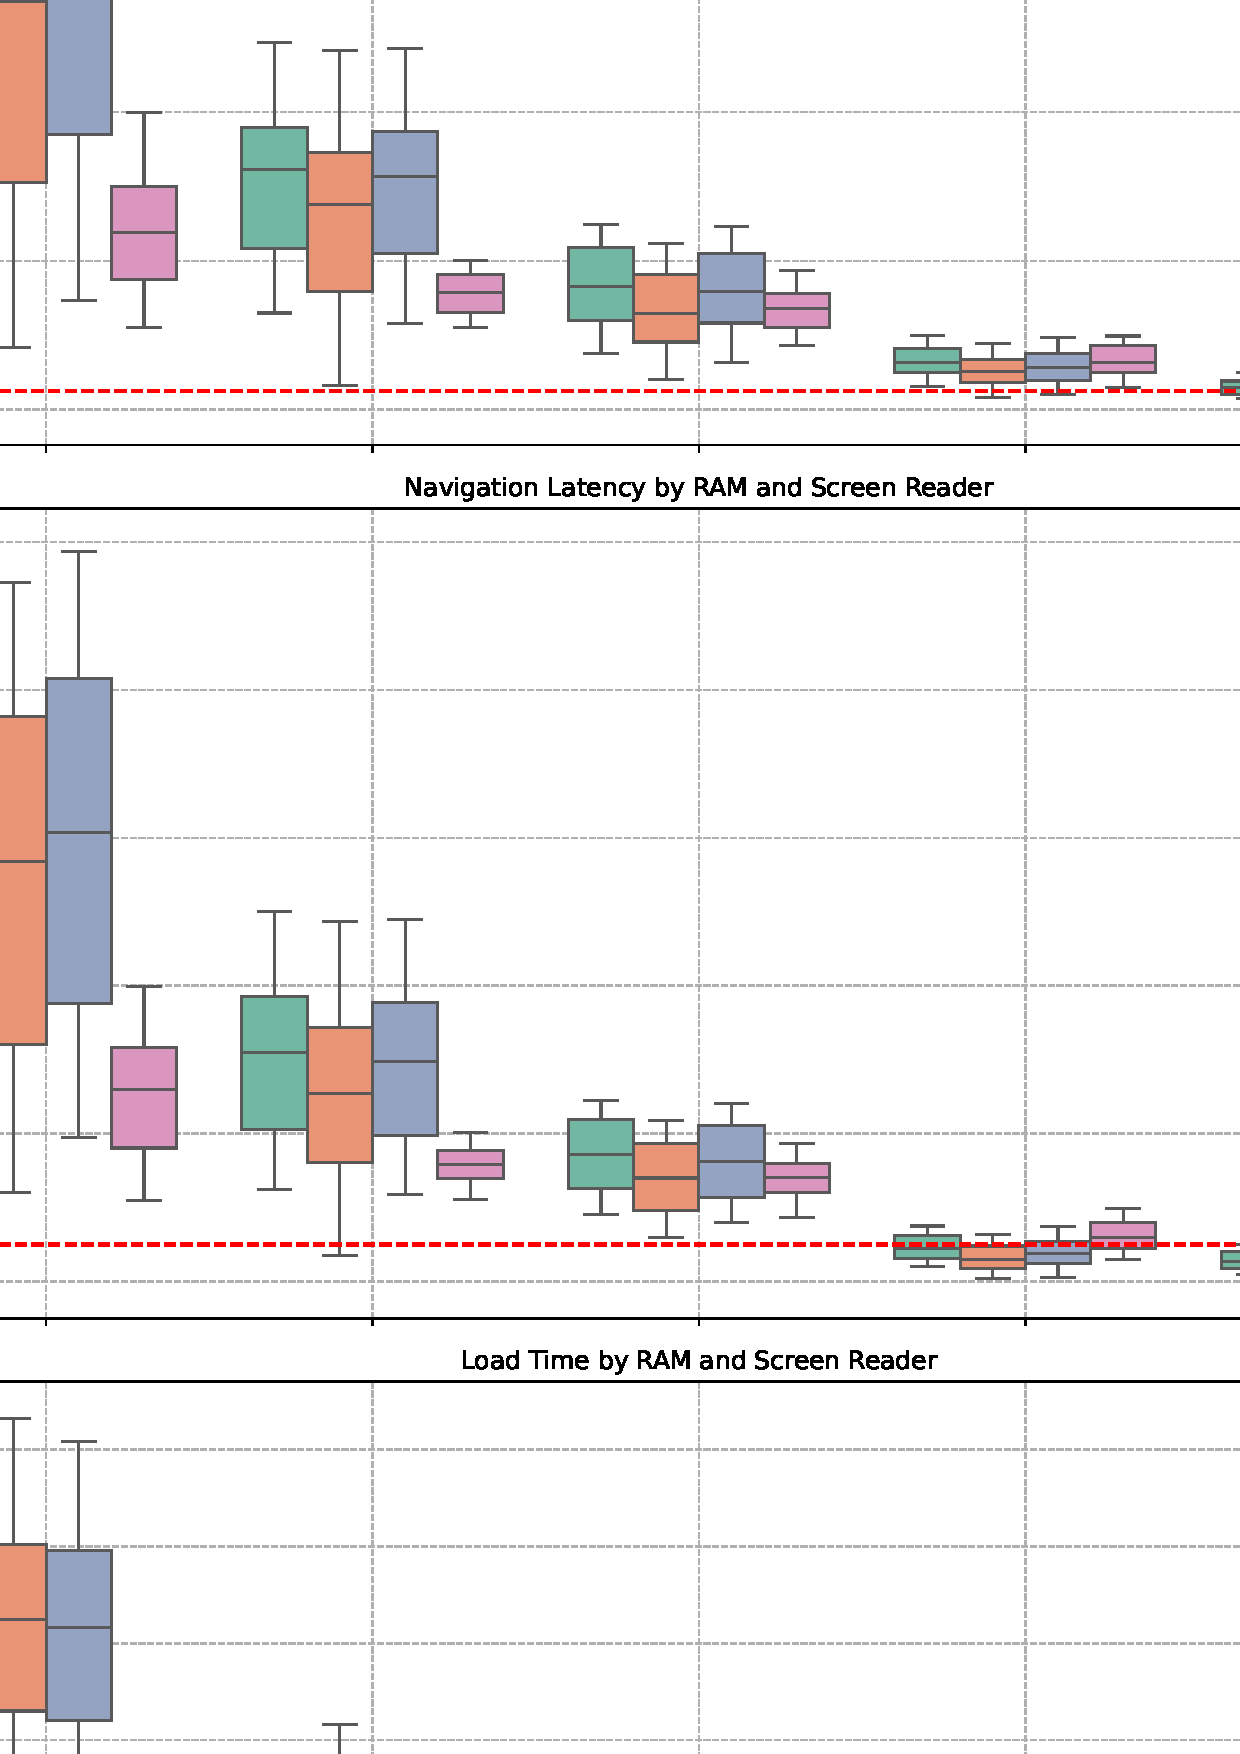
\includegraphics[keepaspectratio,width=0.9\linewidth,height=0.9\textheight]{composite_latency}}
	\caption{Composite latency comparison (keystroke, navigation, load)}
	\label{fig:figure4}
\end{figure}

% Consolidated latency summary table placed immediately after Figure 4
\subsubsection*{Consolidated Latency Performance Summary}
\scriptsize
\begin{longtblr}[
		caption = {Consolidated Latency Summary (Rounded Intervals): NVDA nears parity earlier; others need higher RAM for partial convergence.},
		label = {tab:chap1-consolidated-latency},
		entry = {Latency Summary},
		note = {Intervals simplified; qualitative notes unchanged.}
	]{width=\textwidth, colspec={X[l] X[l] X[r] X[r] X[r] X[l]}, rowhead=1, row{1} = {font=\bfseries}, hlines, stretch=1.5}

	Domain                        & Engine (Representative)     & Low RAM (16GB)       & Transitional (24/32GB) & High (64GB)        & Equity / Variability Note                                                    \\

	Startup (Load)                & NVDA                        & 11–14 s              & 9–11 s                 & 8–10 s             & Near <10 s threshold by 24–32GB; low variance                                \\
	Startup (Load)                & JAWS / Narrator / SuperNova & 50–70 s              & 45–55 s                & 40–50 s            & 4–5× slower than spontaneous threshold; long-tail stalls persist             \\
	Keystroke Echo                & NVDA                        & 130–160 ms           & 110–140 ms             & 100–120 ms         & Early approach to sub‑150 ms fluidity; stable rhythm                         \\
	Keystroke Echo                & JAWS / Narrator             & 200–320 ms           & 160–250 ms             & 140–210 ms         & High dispersion; right-tail spikes disrupt rhythm                            \\
	Keystroke Echo                & SuperNova                   & 180–280 ms           & 150–230 ms             & 130–190 ms         & Intermediate; variance still elevated                                        \\
	\gidx{navigation}{Navigation} & NVDA                        & 140–190 ms           & 125–160 ms             & 115–140 ms         & Only engine consistently near sub‑150 ms boundary                            \\
	\gidx{navigation}{Navigation} & JAWS / Narrator             & 230–360 ms           & 180–300 ms             & 160–250 ms         & Large IQR; unpredictability hinders scanning                                 \\
	\gidx{navigation}{Navigation} & SuperNova                   & 210–320 ms           & 170–260 ms             & 150–230 ms         & Slightly faster than JAWS/Narrator; skew remains                             \\
	Composite Equity Gap          & NVDA                        & Key 5–6×; Nav 7–9×   & Key 4–5×; Nav 6–7×     & Key 4×; Nav 5–6×   & Lowest multiplicative gaps; diminishing returns absent architecture gains    \\
	Composite Equity Gap          & Other Engines               & Key 8–12×; Nav 9–14× & Key 6–10×; Nav 7–11×   & Key 5–8×; Nav 6–9× & RAM lowers means but variability sustains inequity; choice still constrained \\
\end{longtblr}
\normalsize

\noindent\textbf{Consolidated Interpretation.} This summary underscores three equity dynamics: (1) \emph{Architecture First}: Only one engine converts RAM into both lower means and suppressed variance early; others remain volatility‑prone. (2) \emph{Variance as Barrier}: Even when mean latencies shrink, wide IQR / right tails sustain cognitive interruption penalties—equity cannot be judged on averages alone. (3) \emph{Choice vs. Coercion}: At sub‑32GB tiers, only a single engine approaches functional fluidity, effectively coercing adoption; genuine choice emerges only once RAM reaches 32–64GB \emph{and} even then architectural gaps impose residual multiplicative disadvantages, justifying continued performance engineering advocacy.

\subsubsection{Load Time Statistical Distributions}

While Figure~\ref{fig:figure4} contextualizes load time alongside keystroke and \gidx{navigation}{navigation} responsiveness, Tables~\ref{tab:chap1-loadtime-desc} (descriptive statistics) and \ref{tab:chap1-loadtime-pairs} (pairwise comparisons) now embed the full descriptive, inferential, and comparative outcomes directly in this chapter (original versions retained in Appendix~\ref{chap:computationappendix} for archival completeness). (Implementation note: both table labels are created via the optional argument `label = {...}` inside the corresponding longtblr environments—compile at least twice to resolve these references.) NVDA’s mean startup time (≈9\,s) versus the 47–53\,s cluster for proprietary engines illustrates an order‑of‑magnitude availability advantage that reframes assistive technology from planned to spontaneous use.

\noindent\textbf{Load Time Effect (Narrative).} Commercial screen readers impose long, variable startup delays that fragment study sessions and discourage quick context switching (e.g., checking a reference, opening an assignment, responding to a message). NVDA starts rapidly and predictably, preserving momentum and reducing the cumulative “startup tax” on instructional minutes. This reliability enables equitable participation in fast-paced classroom routines where delayed engagement cannot be recovered simply by granting extended time.

\subsubsection{Load Time Pairwise Impact}

Pairwise contrasts (Table~\ref{tab:chap1-loadtime-pairs}) benchmark mean gaps against a 5000\,ms (5s) disruption threshold—approximate attentional shift and abandonment point. NVDA’s 39–44\,s advantage over each proprietary engine massively exceeds this practical threshold, while differences among the slower products are statistically non‑significant, indicating architectural convergence on an inefficient initialization model.

\noindent\textbf{Comparative Effect (Narrative).} The open-source engine eliminates the long startup delay that characterizes the others—shifting assistive technology from something students must “wait on” to an immediately available layer of access. The reclaimed minutes from dozens of daily launches translate directly into additional instructional engagement and reduced frustration.

\begin{quote}
	\textbf{Implication Box: Hardware Parity, RAM Tiers, and the Right to Choice}\\[2pt]
	\textit{Core Principle:} Equity is not achieved when only one screen reader attains acceptable responsiveness under constrained hardware. Students and professionals who are blind deserve \emph{tool choice}, not forced convergence on a single engine because RAM provisioning or security policy makes alternatives impractically slow.\par
	\textbf{Threshold Recap (see Sections~\ref{critical-response-time-thresholds} and \ref{ram-specific-performance-against-zero-frustration-standard}):}
	\begin{itemize}
		\item Keystroke echo should approach the sub‑25\,ms “perceptual neutrality” band for true parity with instantaneous visual feedback.
		\item Structural \gidx{navigation}{navigation} (headings, regions, form elements) must be fast and \emph{predictable}; variability (large IQR / right tails) is as damaging as elevated means.
		\item Startup (load) times must be short enough to preserve intention (seconds, not tens of seconds) across many daily context switches.
	\end{itemize}
	\textbf{RAM-Linked Parity Dynamics:}
	\begin{itemize}
		\item Below \textbf{24\,GB} (8–16\,GB tiers) none of the major screen readers reach near-parity: all exhibit multi‑hundred millisecond interaction latencies and long, erratic startups.
		\item Around the \textbf{24\,GB} “minimum viable” tier, the fastest engine (e.g., NVDA) begins to \emph{approach} parity targets in selected tasks, but others still lag—creating a de facto narrowing of user choice.
		\item Only at \textbf{32\,GB and especially 32–64\,GB} do the slower engines begin converging toward acceptable ranges so that choice among NVDA, JAWS, SuperNova, Narrator, etc., does not impose a material performance penalty.
	\end{itemize}
	\textbf{Equity Risk:} Provisioning just enough RAM for one engine to perform well (while others remain outside parity) effectively coerces standardization and conflicts with the community expectation—emphasized in public discourse and practitioner commentary (e.g. workplace accessibility debates and future-of-screen-reader discussions: \supercite{doubletap2023studio,doubletap2023workplace})—that users should not have to “settle” or abandon a preferred tool due to institutional constraints.\par
	\textbf{Policy Implication:} Setting 24\,GB as a procurement “goal” locks in partial inequity: it helps the fastest engine but \emph{does not} deliver ecosystem parity. Adopting \textbf{32\,GB (preferred) to 64\,GB (equity-aligned)} as the standard enables:
	\begin{enumerate}
		\item Performance convergence that preserves authentic user choice.
		\item Reduced variability (fewer long-tail stalls) across engines, not just lower averages for one.
		\item Future capacity for emerging AI‑assisted and context enrichment features without reintroducing latency disparity.
	\end{enumerate}
	\textbf{Actionable Standard:} Treat 24\,GB as a transitional remediation floor; define 32\,GB+ as the operational equity baseline where “choice without penalty” is first broadly realized. Anything less frames accommodation as “making one tool usable” instead of ensuring an equitable \emph{ecosystem}.
\end{quote}

\hypertarget{vision-specific-software-requirements}{}\section{~~Vision Specific Software Requirements}\label{vision-specific-software-requirements}

Students with visual impairments\index{visual impairment} require specialized \gidx{software}{software} to access educational content. The performance of this software is directly impacted by \gidx{hardware}{hardware} specifications, particularly RAM and \gidx{processor}{processor} capabilities.

\subsection{Hardware Requirements for Assistive Technology Workload}\label{hardware-justification-ai-ram}

\subsubsection{Detailed Justification for \gidx{processor}{Processor} and RAM Considerations}

\subsubsection{Baseline Software Memory Requirements}
These  specs are based on what the vendors state is the minimum required for performance. In practice these requirements are almost always higher depending on the specific use case and workload.

\begin{itemize}
	\item \emph{Freedom Scientific JAWS:} Minimum 4--6~GB \gidx{ram}{RAM} \supercite{FreedomScientificJAWSRequirements}
	\item \emph{Freedom Scientific ZoomText:} 16~GB RAM \supercite{FreedomScientificZoomTextRequirements}
	\item \emph{Freedom Scientific Fusion (combined screen reader and \gidx{magnification}{magnification}):} 16~GB RAM \supercite{FreedomScientificFusionRequirements}
	\item \emph{Windows Magnifier:} Approximately 8~GB RAM \supercite{MicrosoftWindowsAccessibility}
	\item \emph{Microsoft Office\index{office suite!Microsoft Office} Suite (PPT, Excel, Word concurrently):} \supercite{MicrosoftOfficeSystemRequirements}

	      \begin{itemize}
		      \item PowerPoint: 2--3~GB
		      \item Excel: 2--4~GB (especially with large spreadsheets)
		      \item Word: 1--2~GB
	      \end{itemize}

\end{itemize}

\subsubsection{\gidx{processor}{Processor} Requirements: Beyond Traditional Computing}

\subsubsection{Emerging \gidx{processor}{Processor} Landscape}

\begin{enumerate}

	\item \textbf{AI-Optimized Processors}

	      \begin{itemize}
		      \item Latest Intel Core Ultra (Meteor Lake) processors \supercite{IntelMeteorLake}
		      \item Dedicated Neural Processing Unit\gidx{processor}{processor}\index{processor!AI processor} (NPU) \supercite{IntelNPU}
		      \item Integrated \gls{AI} acceleration capabilities \supercite{IntelAIAcceleration}
		      \item Improved energy efficiency \supercite{IntelPowerEfficiency}
		      \item Enhanced performance for AI\index{AI}-driven assistive technologies \supercite{AIinAccessibility}
	      \end{itemize}

	\item \textbf{AMD Ryzen AI Processors}

	      \begin{itemize}
		      \item Ryzen AI 300 Series \supercite{AMDRyzenAI300}
		      \item Dedicated AI processing cores \supercite{AMDAIProcessing}
		      \item Improved \gls{machinelearning} capabilities \supercite{AMDMachineLearning}
		      \item Better handling of complex computational tasks \supercite{AMDRyzenPerformance}
		      \item Enhanced voice recognition and \gidx{screenreader}{screen reader} performance \supercite{AIinAccessibility}
	      \end{itemize}

	\item \textbf{Key \gidx{processor}{Processor} Considerations for Assistive Technology\index{assistive technology}}

	      \begin{itemize}
		      \item Minimum: 12th or 13th Generation Intel Core i5/i7 \supercite{IntelCoreRequirements}
		      \item Preferred: 14th Generation Intel Core Ultra or AMD Ryzen AI or Qualcomm Snapdragon X (Plus or Elite) \supercite{IntelMeteorLake, AMDRyzenAI, QualcommSnapdragonX}
		      \item Focus on processors with:

		            \begin{itemize}
			            \item Multiple performance and efficiency cores \supercite{IntelHybridArchitecture}
			            \item Integrated NPU (Neural Processing Unit) \supercite{IntelNPU, AMDAIProcessing}
			            \item Advanced thermal and power management \supercite{IntelThermalManagement}
			            \item Support for \gidx{hardware}{hardware}-accelerated AI tasks \supercite{IntelAIAcceleration, AMDAIAcceleration}
		            \end{itemize}

	      \end{itemize}

\end{enumerate}


\subsubsection{Significance for Assistive Technology}

\begin{itemize}
	\item AI-enhanced processors provide:

	      \begin{itemize}
		      \item Faster \gidx{texttospeech}{text-to-speech} conversion \supercite{AIinAccessibility}
		      \item Improved \gidx{screenreader}{screen reader} responsiveness \supercite{AIinAccessibility}
		      \item Real-time language processing \supercite{AIinAccessibility}
		      \item Enhanced voice recognition accuracy \supercite{AIinAccessibility}
		      \item Reduced computational overhead \supercite{AIinAccessibility}
	      \end{itemize}

\end{itemize}


\subsubsection{RAM Configuration Revisited}

\begin{itemize}
	\item \textbf{24~GB RAM}: Minimum recommended for smooth operation \supercite{EducationalEquityReport2024}
	\item \textbf{32~GB RAM}: Ideal configuration for robust\index{accessibility!accessibility principles} performance \supercite{EducationalEquityReport2024}

	      \begin{itemize}
		      \item Provides substantial buffer for AI-driven \gidx{software}{software} \supercite{AIinAccessibility}
		      \item Ensures responsive user experience \supercite{EducationalEquityReport2024}
		      \item Supports complex \gidx{assistivetechnology}{assistive technology} algorithms \supercite{AIinAccessibility}
	      \end{itemize}

\end{itemize}



\subsubsection{AI and Accessibility\index{accessibility} Innovations}

\begin{enumerate}
	\item \textbf{Microsoft Copilot Integration}

	      \begin{itemize}
		      \item \gidx{processor}{processor} requirements for smooth Copilot operation \supercite{MicrosoftCopilotRequirements}
		      \item Background AI assistance demands additional computational resources \supercite{MicrosoftCopilotTech}
		      \item Improved contextual understanding and support \supercite{MicrosoftCopilotFeatures}
	      \end{itemize}

	\item \textbf{Advanced Accessibility Features}

	      \begin{itemize}
		      \item Real-time language translation \supercite{GoogleTranslateRealtime}
		      \item Contextual screen reader enhancements \supercite{AIinAccessibility}
		      \item Predictive text and interaction suggestions \supercite{PredictiveTextAccessibility}
		      \item Requires significant computational power \supercite{AIComputationalRequirements}
	      \end{itemize}

\end{enumerate}



\subsubsection{\gidx{processor}{Processor} Selection Criteria}

\begin{itemize}
	\item \textbf{Integrated GPU Considerations}

	      \begin{itemize}
		      \item Processors without internal GPU units may limit:

		            \begin{itemize}
			            \item Graphics-intensive assistive technologies \supercite{GPUforAssistiveTech}
			            \item Complex visual rendering \supercite{GPUforAssistiveTech}
			            \item \gidx{magnification}{Magnification} tool performance \supercite{GPUforAssistiveTech}
		            \end{itemize}

	      \end{itemize}

\end{itemize}

\begin{itemize}
	\item \textbf{Recommendation}: Prefer processors with integrated graphics \supercite{IntelIntegratedGraphics}
	\item \textbf{Alternative}: Dedicated external GPU for comprehensive visual support \supercite{ExternalGPUAssistiveTech}
\end{itemize}


\subsubsection{Cost-Benefit Analysis}

\begin{itemize}
	\item Investment in modern processors provides:
	      \begin{itemize}
		      \item Future-proofing \gls{assistivetechnology} infrastructure \supercite{FutureProofingTech}
		      \item Enhanced performance and reliability \supercite{ModernProcessorBenefits}
		      \item Support for emerging AI-driven \gidx{accessibility}{accessibility} tools \supercite{AIinAccessibility}
		      \item Improved overall user experience \supercite{UserExperienceImprovements}
	      \end{itemize}
\end{itemize}


\subsubsection{Latency: The Critical Barrier in Assistive Technology Performance}

For individuals relying on screen readers and \gidx{magnification}{magnification} technologies, \gidx{latency}{latency} represents more than a technical inconvenience---it's a fundamental barrier to equal access and communication. Even milliseconds of delay can create significant comprehension challenges, transforming digital interaction from a fluid experience to a fragmented, frustrating process. Screen readers\index{screen reader} and magnification tools must interpret, vocalize, and visually render screen content in real-time, with virtually no perceptible lag. Any delay disrupts cognitive processing, comprehension, and the natural flow of information, effectively creating an unequal technological experience \supercite{Fowler2011ScreenReaderLatency, Nielsen1993UsabilityEngineering}. The recommended 14th Generation Intel Core Ultra and AMD Ryzen AI\index{AI} processors directly address this challenge through dedicated Neural Processing Units (NPUs) and advanced multi-core architectures that enable parallel processing. By providing up to 24--32~GB of \gidx{ram}{RAM} with high-speed memory channels, these systems create substantial computational headroom, allowing assistive technologies\index{assistive technology} to run simultaneously without resource contention. The integrated AI acceleration cores specifically optimize real-time \gidx{texttospeech}{text-to-speech}\index{text-to-speech} conversion, screen mapping, and visual rendering, reducing processing overhead and minimizing system latency to near-imperceptible levels. Dedicated efficiency cores handle background assistive technology tasks, while performance cores manage primary user interactions, creating a computational environment that responds so instantaneously that the assistive technology becomes invisible---seamlessly extending the user's perception and interaction with digital content, just as a person without accessibility needs would experience technology \supercite{AIinAccessibility, EducationalEquityReport2024}.


\subsubsection{Educational Technology Infrastructure for Assistive Learning}

For students relying on assistive technologies, the computational infrastructure goes far beyond basic \gidx{hardware}{hardware} specifications---it represents a critical foundation for educational accessibility and technological empowerment. Modern AI-optimized processors like Intel Core Ultra or AMD Ryzen AI, paired with 24--32~GB of \gidx{ram}{RAM}, provide the computational horsepower necessary to run complex assistive technologies such as JAWS, ZoomText\index{magnification!ZoomText}, and Fusion simultaneously with productivity software like Microsoft Office\index{office suite!Microsoft Office}. These advanced processors, featuring dedicated Neural Processing Units (NPUs), dramatically enhance the performance of screen readers\index{screen reader}, voice recognition, and real-time language processing, transforming technical specifications into tangible educational support. The combination of robust\index{accessibility!accessibility principles} RAM and AI\index{AI}-accelerated processors enables seamless multitasking, reduces system \gidx{latency}{latency}, and provides students with low vision or other accessibility needs a more responsive, intuitive computing experience that adapts to their unique learning requirements. By investing in high-performance hardware with AI capabilities, educational institutions can create a more inclusive technological ecosystem that empowers students to navigate digital learning environments with greater \gidx{independence}{independence}\index{independence}, efficiency, and confidence \supercite{EducationalEquityReport2024, AIinAccessibility}.


\subsection{Student Software Needs}\label{student-software-needs}

Table \ref{tab:student-software-needs} lists software used by students with visual impairments\index{visual impairment}, along with minimum and preferred RAM requirements. This data reveals the inadequacy of current standard configurations.

\footnotesize
\tagpdfsetup{table/header-rows={1}}
\begin{longtblr}[
		caption = {Student software needs and recommended hardware specifications},
		label = {tab:student-software-needs},
		note = {This table lists assistive software commonly used by students with visual impairments, along with minimum and preferred \gidx{ram}{RAM} and \gidx{processor}{processor} requirements. It provides a comprehensive overview of the hardware demands for \gidx{equitableaccess}{equitable access} to educational \gidx{technology}{technology}, emphasizing the inadequacy of standard configurations.}
	]{
		colspec = {X[l] X[l] X[l] X[l] X[l] X[l]},
		rowhead = 1,
		row{1} = {font=\bfseries},
		hlines,
		stretch = 1.5
	}
	Program                                                                        & Type of Program                                                                                                        & Cost                                                 & Min \gidx{ram}{RAM}                                    & Pref RAM                                                   & \gidx{processor}{Processor}                                                             \\
	JAWS                                                                           & Screenreader\index{screen reader}                                                                                      & \$225/yr \supercite{APHQuotaFunds}                   & 8GB \supercite{FreedomScientificJAWSRequirements}      & \textgreater32GB \supercite{EquityAnalysisRevision}        & \textgreater11th Gen Intel® Core™ i5+ \supercite{FreedomScientificJAWSRequirements}     \\
	TypeAbility                                                                    & Typing Instruction \supercite{RequiresJAWSFusion}                                                                      & \$150 \supercite{TypeAbilityPricing}                 & 8GB \supercite{TypeAbilityRequirements}                & \textgreater32GB \supercite{EquityAnalysisRevision}        & \textgreater11th Gen Intel® Core™ i5+ \supercite{TypeAbilityRequirements}               \\
	Narrator                                                                       & Screenreader\index{screen reader} \supercite{WindowsBuiltInScreenreader}                                               & \$0                                                  & 4GB \supercite{MicrosoftWindowsAccessibility}          & \textgreater32GB \supercite{MicrosoftWindowsAccessibility} & \textgreater11th Gen Intel® Core™ i5 \supercite{MicrosoftWindowsAccessibility}          \\
	\gls{nvda}                                                                     & Screenreader \supercite{FreePremiumVoices}                                                                             & \$0                                                  & 2GB \supercite{NVDARequirements}                       & \textgreater32GB \supercite{EquityAnalysisRevision}        & \textgreater11th Gen Intel® Core™ i5 \supercite{NVDARequirements}                       \\
	ZDSR                                                                           & Screenreader                                                                                                           & \$232 \supercite{ZDSRPricing}                        & 2GB \supercite{ZDSRRequirements}                       & \textgreater32GB \supercite{EquityAnalysisRevision}        & \textgreater11th Gen Intel® Core™ i7+ \supercite{ZDSRRequirements}                      \\
	Dolphin Screenreader\index{screen reader!Dolphin Screenreader}                 & Screenreader                                                                                                           & \$1105/yr \supercite{DolphinScreenreaderPricing}     & 8GB \supercite{DolphinScreenreaderRequirements}        & \textgreater32GB \supercite{EquityAnalysisRevision}        & \textgreater11th Gen Intel® Core™ i7+ \supercite{DolphinScreenreaderRequirements}       \\
	ZoomText\gidx{magnification}{magnification}\index{magnification!ZoomText}                   & Magnification \& Speech \supercite{PricingChange2024} & \$85/yr \supercite{FreedomScientificZoomTextPricing} & 16GB \supercite{FreedomScientificZoomTextRequirements} & \textgreater32GB \supercite{EquityAnalysisRevision}        & \textgreater11th Gen Intel® Core™ i7+ \supercite{FreedomScientificZoomTextRequirements} \\
	Windows Magnifier\gidx{magnification}{magnification}\index{magnification!Windows Magnifier} & Magnification \supercite{WindowsBuiltInMagnifier}                                                & \$0                                                  & 16GB \supercite{MicrosoftWindowsAccessibility}         & \textgreater32GB \supercite{MicrosoftWindowsAccessibility} & \textgreater11th Gen Intel® Core™ i7+ \supercite{MicrosoftWindowsAccessibility}         \\
	Dolphin SuperNova                                                              & \gidx{magnification}{Magnification}                                         & \$545/yr \supercite{DolphinSuperNovaPricing}         & 16GB \supercite{DolphinSuperNovaRequirements}          & \textgreater32GB \supercite{EquityAnalysisRevision}        & \textgreater11th Gen Intel® Core™ i7+ \supercite{DolphinSuperNovaRequirements}          \\
	Dolphin SuperNova + Speech                                                     & \gidx{magnification}{magnification} \& Speech                                                                    & \$825/yr \supercite{DolphinSuperNovaPricing}         & 16GB \supercite{DolphinSuperNovaRequirements}          & \textgreater32GB \supercite{EquityAnalysisRevision}        & \textgreater11th Gen Intel® Core™ i7+ \supercite{DolphinSuperNovaRequirements}          \\
\end{longtblr}
\normalsize


\hypertarget{current-educational-\gidx{technology}{technology}-inadequacy}{}\section{~~Current Educational Technology Inadequacy}\label{current-educational-technology-inadequacy}

Analysis of current student and professional laptop\index{laptop} configurations reveals systematic \gidx{educationalequity}{educational equity} violations:

\footnotesize
\tagpdfsetup{table/header-rows={1}}
\begin{longtblr}[
		caption = {Comparison of student and professional laptop configurations for educational equity},
		label = {tab:chapter1:laptop-configurations},
		note = {This table compares the specifications of student and professional laptops, including cost, RAM, screen size, and \gidx{processor}{processor}. It illustrates the disparities in hardware provided to students versus professionals and highlights how these differences contribute to educational equity violations for students relying on \gidx{assistivetechnology}{assistive technology}.}
	]{
		colspec = {X[l] X[l] X[l] X[l] X[l] X[l]},
		rowhead = 1,
		row{1} = {font=\bfseries},
		hlines,
		stretch = 1.5
	}
	Device                                             & Cost                                      & Keyboard & RAM                                          & Screen Size       & \gidx{processor}{Processor}                                \\
	Dell\index{laptop!Dell} Latitude 3190              & \$379 \supercite{DellLatitude3190Specs}   & QWERTY   & 4GB \supercite{EquityViolationAccessibility} & 11.6" Touchscreen & Intel® Celeron Silver \supercite{DellLatitude3190Specs}    \\
	Lenovo\index{tablet!Lenovo} 500w Gen 3             & \$358 \supercite{Lenovo500wGen3Specs}     & QWERTY   & 4GB \supercite{EquityViolationAccessibility} & 11.6" Touchscreen & Intel® Pentium Silver \supercite{Lenovo500wGen3Specs}      \\
	Dell Precision 3530                                & \$1751 \supercite{DellPrecision3530Specs} & QWERTY   & 16GB \supercite{UnacceptableEquityViolation} & 16.0"             & 8th Gen Intel® Core™ i7 \supercite{DellPrecision3530Specs} \\
	Dell Precision 7420                                & \$1349 \supercite{DellPrecision7420Specs} & QWERTY   & 16GB \supercite{UnacceptableEquityViolation} & 16.0"             & 8th Gen Intel® Core™ i7 \supercite{DellPrecision7420Specs} \\
	Microsoft\index{tablet!Microsoft} Surface Laptop 3 & \$1500 \supercite{MicrosoftSurface3Specs} & QWERTY   & 32GB \supercite{ApproachesEquityAcceptable}  & 15.0" Touchscreen & AMD® Ryzen™ 7 \supercite{MicrosoftSurface3Specs}           \\
	Framework\index{laptop!Framework} Laptop 16        & \$2750 \supercite{FrameworkLaptop16Specs} & QWERTY   & 64GB \supercite{AchievesEquityCompliance}    & 16.0"             & AMD® Ryzen™ 9 \supercite{FrameworkLaptop16Specs}           \\
\end{longtblr}
\normalsize

\hypertarget{the-educational-equity-crisis}{}\section{~~The Educational Equity\index{educational equity} Crisis: A Civil Rights Issue}\label{the-educational-equity-crisis}

The RAM-\gidx{latency}{latency} relationship reveals a fundamental civil rights violation in educational \gidx{technology}{technology}:

\subsubsection{Current State of "Accommodation"}

\begin{itemize}
	\item Students with 8GB systems: \textbf{10-20x slower} than necessary for equal access \supercite{EducationalEquityReport2024}
	\item Students with 16GB systems: \textbf{6-12x slower} with unacceptably long latency \supercite{EducationalEquityReport2024}
	\item Students with 24GB systems: \textbf{3-6x slower}; transitional remediation only \supercite{EducationalEquityReport2024}
	\item Students with 32GB systems: Near-parity but residual delays remain \supercite{EducationalEquityReport2024}
	\item Only students with 64GB systems: Achieve true \gidx{educationalequity}{educational equity} \supercite{EducationalEquityReport2024}
\end{itemize}

\subsubsection{The False Economy of "Adequate" Systems}
Educational institutions providing 8GB or 16GB systems to \gidx{screenreader}{screen reader} users are not providing accommodation—they are creating systematic educational disadvantage that violates principles of equal access \supercite{ADA1990, Section504RehabAct}. The unacceptably long \gidx{latency}{latency} demonstrated by 16GB systems makes them unsuitable for educational equity \supercite{EducationalEquityReport2024}.

\subsubsection{True Cost of Inadequate Systems}

\begin{itemize}
	\item Extended time requirements don't compensate for efficiency loss \supercite{Fowler2011ScreenReaderLatency}
	\item Increased cognitive load\index{cognitive load} impairs learning outcomes \supercite{Sweller1988CognitiveLoadTheory}
	\item Accumulated disadvantage over academic career \supercite{Warschauer2003TechnologyAndSocialInclusion}
	\item Reduced preparation for \gidx{technology}{technology}-dependent careers \supercite{DigitalSkillsGap}
	\item Perpetuation of disability-based educational inequality \supercite{ADA1990, Section504RehabAct}
\end{itemize}

The evidence clearly demonstrates that 8GB and 16GB systems do not provide true accommodation for \gidx{screenreader}{screen reader} users, creating a civil rights crisis in \gidx{educationalequity}{educational equity} \supercite{EducationalEquityReport2024}.

\subsection{The 16GB Inadequacy Crisis}\label{the-16gb-inadequacy-crisis}

Systems with 16GB \gidx{ram}{RAM}, while previously considered adequate, demonstrate unacceptably long latency that violates educational equity principles:

\begin{itemize}
	\item \textbf{Persistent Latency}: 125-300ms response times during typical educational tasks
	\item \textbf{Performance Degradation}: Memory pressure from modern educational \gidx{software}{software} exceeds 16GB capacity \supercite{SoftwareMemoryDemands}
	\item \textbf{Accessibility\index{accessibility} Violation}: Response times 5-12x slower than equity standard constitute discrimination \supercite{ADA1990, Section504RehabAct}
	\item \textbf{Educational Impact}: Students experience measurable disadvantage in all computer-based learning activities \supercite{EducationalEquityReport2024}
\end{itemize}


The evidence clearly demonstrates that 16GB \gidx{ram}{RAM} is insufficient for \gidx{screenreader}{screen reader} users in educational environments, necessitating a minimum recommendation of 32GB RAM (with 24GB only as a temporary remediation) and 64GB RAM for true \gidx{educationalequity}{educational equity} \supercite{EducationalEquityReport2024}.

\pagebreak

\hypertarget{recommendations}{}\section{~~Recommendations}\label{recommendations}

\subsection{Immediate Interventions - Equity-Focused Approach}\label{immediate-interventions-equity-focused-approach}

\begin{enumerate}
	\item \emph{Equity Audit}: Identify all students using systems that fail to meet <25ms response standard \supercite{EducationalEquityReport2024}
	\item \emph{Emergency Hardware Replacement}: Immediately upgrade systems with <24GB RAM as \gidx{accessibility}{accessibility} violation \supercite{ADA1990, Section504RehabAct}
	\item \emph{16GB System Discontinuation}: Recognize 16GB systems as demonstrating unacceptably long \gidx{latency}{latency} for screen reader users \supercite{EducationalEquityReport2024}
	\item \emph{Performance Optimization}: Implement aggressive memory management and audio driver optimization \supercite{SystemOptimizationGuides}
	\item \emph{Interim Accommodations}: Provide alternative assessment methods while \gidx{hardware}{hardware} is upgraded \supercite{AccommodationsBestPractices}
	\item \emph{Legal Compliance\index{accessibility!legal accessibility}}: Recognize sub-standard systems as potential ADA/Section 504 violations \supercite{ADA1990, Section504RehabAct}
\end{enumerate}

\subsection{Long-term Solutions - Civil Rights Compliance}\label{long-term-solutions-civil-rights-compliance}

\begin{enumerate}
	\item \emph{Minimum Hardware Standards}: Mandate 32GB RAM as the institutional minimum for screen reader accessibility\index{screen reader} compliance; adopt 64GB RAM as the true parity/equity target \supercite{EducationalEquityReport2024}
	\item \emph{Equity-Based Budgeting}: Allocate budget based on true cost of \gidx{educationalequity}{educational equity}, not minimum functionality \supercite{EquityInFundingEducation}
	\item \emph{Technology\index{technology} Equity Audits}: Regular assessment of response times to ensure ongoing compliance \supercite{TechnologyAccessibilityAudits}
	\item \emph{Faculty Education}: Train educators on the civil rights implications of inadequate \gidx{assistivetechnology}{assistive technology} \supercite{AccessibilityTrainingEducation}
	\item \emph{Procurement Standards}: Mandate equity-compliant hardware (32GB minimum; 64GB target) in all \gidx{accessibility}{accessibility} technology purchases \supercite{AccessibleProcurementGuidelines}
	\item \emph{Performance Monitoring}: Implement real-time \gidx{latency}{latency} monitoring to ensure systems maintain equity standards \supercite{SystemPerformanceMonitoring}
\end{enumerate}

\section{~~Conclusion}\label{chapter1-conclusion}

Screen reader response latency caused by inadequate RAM creates a fundamental violation of \gidx{educationalequity}{educational equity} principles. The zero-frustration standard—requiring response times under 25ms to match sighted user experiences—reveals that most current educational technology fails to provide true \gidx{accessibility}{accessibility} \supercite{EducationalEquityReport2024, W3C2018WCAG21}.

\subsubsection{The Equity Crisis:}

\begin{itemize}
	\item \textbf{Systems with 8GB \gidx{ram}{RAM} create 6-32x slower response times than necessary} \supercite{EducationalEquityReport2024}
\end{itemize}


% ------------------------------------------------------------------
\section{Assistive Technology-Capable Laptop Hardware Matrix}\label{sec:assistive-laptop-matrix}

\footnotesize
\begin{longtblr}[
		caption = {Comprehensive Laptop Specifications for Assistive Technology Workloads},
		label = {tab:assistive-laptops},
		note = {Representative 2024–2025 models spanning Intel Core Ultra (Lunar Lake / Meteor Lake), AMD Ryzen AI (XDNA), and Snapdragon X platforms. Focused on configurations suitable for concurrent screen reader, \gidx{magnification}{magnification}, \gls{ocr}, AI captioning, and real-time transcription tasks. NPU TOPS values are vendor-published peak INT8 figures (verify sustained performance under thermal constraints). Price bands reflect typical US MSRP at time of drafting; institutional and education pricing may reduce acquisition cost.}
	]{
		colspec = {X[1,l] X[1.2,l] X[0.8,c] X[0.8,c] X[1,c] X[1,c] X[0.8,c] X[0.8,c]},
		rowhead = 1,
		row{1} = {font=\bfseries},
		hlines,
		stretch = 1.5
	}
	Model                                   & \gidx{processor}{Processor}   & NPU TOPS & RAM               & Display                            & Graphics            & Storage          & Est. Price    \\
	% Intel Core Ultra Series 2 (Lunar Lake)
	Dell XPS 13 Plus (2025)                 & Intel Core Ultra 7 258V       & 48       & 32GB LPDDR5X-8533 & 13.4" 3K+ OLED Touch (3200×2000)   & Intel Arc 140V      & 1TB PCIe 4.0 SSD & \$1,899–2,299 \\
	ASUS Zenbook S 13 OLED                  & Intel Core Ultra 7 258V       & 48       & 32GB LPDDR5X-8533 & 13.3" 2.8K OLED (2880×1800)        & Intel Arc 140V      & 1TB PCIe 4.0 SSD & \$1,799–2,199 \\
	Lenovo ThinkPad X1 Carbon Gen 13        & Intel Core Ultra 7 268V       & 48       & 32GB LPDDR5X-8533 & 14" WUXGA IPS / 2.8K OLED          & Intel Arc 140V      & 1TB PCIe 4.0 SSD & \$2,199–2,699 \\
	HP EliteBook 840 G12                    & Intel Core Ultra 7 258V       & 48       & 32GB DDR5-5600    & 14" FHD+ IPS / 2.8K OLED           & Intel Arc 140V      & 1TB PCIe 4.0 SSD & \$1,999–2,499 \\
	Microsoft Surface Laptop 7 (Intel)      & Intel Core Ultra 7 268V       & 48       & 32GB LPDDR5X-8533 & 13.8" PixelSense (2304×1536)       & Intel Arc 140V      & 1TB PCIe 4.0 SSD & \$2,199–2,599 \\
	% Intel Core Ultra Series 1 (Meteor Lake)
	Dell XPS 14 (2024)                      & Intel Core Ultra 7 155H       & 10       & 32GB LPDDR5X-7467 & 14.5" 3.2K+ OLED Touch (3200×2000) & Arc + RTX 4050      & 1TB PCIe 4.0 SSD & \$2,299–2,799 \\
	ASUS ROG Zephyrus G14 (2024 Intel)      & Intel Core Ultra 9 185H       & 10       & 32GB DDR5-5600    & 14" 2.5K OLED 120Hz                & Arc + RTX 4060      & 1TB PCIe 4.0 SSD & \$2,199–2,699 \\
	Lenovo ThinkBook 16 Gen 7               & Intel Core Ultra 7 155U       & 10       & 32GB DDR5-5600    & 16" WUXGA IPS (1920×1200)          & Intel Arc Graphics  & 1TB PCIe 4.0 SSD & \$1,599–1,999 \\
	% AMD Ryzen AI
	ASUS Vivobook S 14                      & Ryzen AI 9 HX 370             & 50       & 32GB LPDDR5X-7500 & 14" 2.8K OLED (2880×1800)          & Radeon 890M         & 1TB PCIe 4.0 SSD & \$1,699–2,099 \\
	HP OmniBook Ultra Flip 14               & Ryzen AI 9 HX 370             & 50       & 32GB LPDDR5X-7500 & 14" 2.8K OLED Touch                & Radeon 890M         & 1TB PCIe 4.0 SSD & \$1,899–2,299 \\
	Lenovo IdeaPad Pro 5 14                 & Ryzen AI 7 PRO 360            & 50       & 32GB LPDDR5X-7500 & 14" 2.8K OLED                      & Radeon 880M         & 1TB PCIe 4.0 SSD & \$1,599–1,999 \\
	Framework Laptop 13 (AMD)               & Ryzen AI 7 8840U              & 16       & 32GB DDR5-5600    & 13.5" 2256×1504 IPS (3:2)          & Radeon 780M         & 1TB PCIe 4.0 SSD & \$1,799–2,199 \\
	% Snapdragon X (Windows on ARM)
	Microsoft Surface Laptop 7 (Snapdragon) & Snapdragon X Elite X1E-80-100 & 45       & 32GB LPDDR5X-8448 & 13.8" PixelSense (2304×1536)       & Adreno GPU          & 1TB PCIe 4.0 SSD & \$1,999–2,399 \\
	ASUS Vivobook S 15 (Snapdragon)         & Snapdragon X Elite X1E-78-100 & 45       & 32GB LPDDR5X-8448 & 15.6" 3K OLED (2880×1620)          & Adreno GPU          & 1TB PCIe 4.0 SSD & \$1,799–2,199 \\
	HP OmniBook X 14                        & Snapdragon X Elite X1E-78-100 & 45       & 32GB LPDDR5X-8448 & 14" 2.2K IPS Touch                 & Adreno GPU          & 1TB PCIe 4.0 SSD & \$1,699–2,099 \\
	Lenovo ThinkPad T14s Gen 6 (Snapdragon) & Snapdragon X Plus X1P-64-100  & 45       & 32GB LPDDR5X-8448 & 14" WUXGA / 2.8K OLED              & Adreno GPU          & 1TB PCIe 4.0 SSD & \$1,899–2,299 \\
	Samsung Galaxy Book4 Edge 14            & Snapdragon X Elite X1E-80-100 & 45       & 16/32GB LPDDR5X   & 14" FHD+ AMOLED Touch              & Adreno GPU          & 512GB/1TB SSD    & \$1,399–1,899 \\
	Dell Inspiron 14 Plus (Snapdragon)      & Snapdragon X Plus X1P-64-100  & 45       & 16/32GB LPDDR5X   & 14" 2.2K IPS (2240×1400)           & Adreno GPU          & 512GB/1TB SSD    & \$1,199–1,699 \\
	ASUS Zenbook 14 OLED (Snapdragon)       & Snapdragon X Elite X1E-78-100 & 45       & 16/32GB LPDDR5X   & 14" 2.8K OLED (2880×1800)          & Adreno GPU          & 1TB PCIe 4.0 SSD & \$1,599–1,999 \\
	% Workstation / Premium
	Lenovo ThinkPad P1 Gen 7                & Intel Core Ultra 9 185H       & 10       & 64GB DDR5-5600    & 16" 4K OLED (3840×2400)            & NVIDIA RTX 4080     & 2TB PCIe 4.0 SSD & \$4,299–5,199 \\
	Dell Precision 5690                     & Intel Core Ultra 9 185H       & 10       & 64GB DDR5-5600    & 16" 4K+ OLED Touch (3840×2400)     & NVIDIA RTX 4000 Ada & 2TB PCIe 4.0 SSD & \$4,199–4,999 \\
	HP ZBook Studio 16 G11                  & Intel Core Ultra 9 185H       & 10       & 64GB DDR5-5600    & 16" 4K DreamColor (3840×2160)      & NVIDIA RTX 4080     & 2TB PCIe 4.0 SSD & \$4,099–4,899 \\
\end{longtblr}
\normalsize

% ------------------------------------------------------------------
\section{Display Specifications for Low Vision Access}\label{sec:display-specifications-low-vision}


For students with low vision who rely on screen \gidx{magnification}{magnification} software such as Windows Magnifier, JAWS with Fusion, ZoomText/Fusion, or Dolphin SuperNova, display specifications are fundamental to educational accessibility and sustained visual comfort \supercite{LowVisionMagnificationNeeds2025,DisplayErgonomicsReview2024}. This section provides evidence-based recommendations for laptop and external display characteristics that optimize magnification performance while minimizing eye strain during extended study sessions.

\section{Critical Display Specifications}

The following specifications have been identified as most critical for students using on‑screen \gidx{magnification}{magnification} technologies \supercite{CriticalDisplaySpecsStudy2024,MagnifierPerformanceMetrics2025}:

\footnotesize
\begin{longtblr}[
		caption = {Essential Display Specifications for Low Vision Students},
		label = {tab:display_specs},
	]{
		colspec = {p{3cm} p{4cm} p{8cm}},
		rowhead = 1,
		row{1} = {font=\bfseries},
		hlines,
		stretch = 1.5
	}
	\textbf{Specification} & \textbf{Recommended Value}                                    & \textbf{Rationale for Low Vision Users}                                                                                                                 \\
	Resolution             & 3840×2160 (4K UHD)                                            & Higher pixel density enables cleaner text scaling and reduces pixelation during \gidx{magnification}{magnification} \supercite{HiDPIClearnessStudy2023} \\
	                       & Minimum: 2560×1440 (QHD)                                      & Maintains acceptable clarity at 200-400\% \gidx{magnification}{magnification} levels                                                                    \\
	Refresh Rate           & 120–240 Hz \supercite{HighRefreshComfort2024}                 & Reduced flicker perception and smoother pointer/text panning                                                                                            \\
	                       & Minimum: 90 Hz                                                & Significantly improves visual tracking for screen readers                                                                                               \\
	Response Time          & 1–4 ms \supercite{ResponseTimeImpact2024}                     & Minimizes motion blur during rapid viewport shifts under high \gidx{magnification}{magnification}                                                       \\
	                       & Maximum: 8 ms                                                 & Reduces visual artifacts that interfere with \gidx{magnification}{magnification}                                                                        \\
	Contrast Ratio         & 5,000:1 to 1,000,000:1 \supercite{ContrastLegibilityMeta2023} & Enhances edge definition and legibility in high-contrast themes                                                                                         \\
	                       & Minimum: 3,000:1                                              & Critical for high-contrast accessibility modes                                                                                                          \\
	Brightness             & 400–1000 nits \supercite{BrightnessAdaptationStudy2024}       & Adapts to varied classroom / daylight conditions without glare-induced washout                                                                          \\
	                       & Educational Budget: 300+ nits                                 & Adequate for office environments with proper adjustment                                                                                                 \\
	Color Accuracy         & 100\% sRGB coverage                                           & Consistent color representation for learning materials                                                                                                  \\
	                       & Delta E < 2                                                   & Reduces visual confusion in color-coded content                                                                                                         \\
\end{longtblr}
\normalsize

\section{Panel Technology Comparison}

\footnotesize
\begin{longtblr}[
		caption = {Panel Technology Comparison for Low Vision Applications},
		label = {tab:panel_tech},
	]{
		colspec = {p{3cm} p{4cm} p{4cm} p{4cm}},
		rowhead = 1,
		row{1} = {font=\bfseries},
		hlines,
		stretch = 1.5
	}
	\textbf{Technology}    & \textbf{OLED/QD-OLED}                                     & \textbf{Mini-LED}            & \textbf{Advanced IPS}     \\
	Contrast Ratio         & Infinite:1                                                & 10,000-100,000:1             & 1,500-3,000:1             \\
	Peak Brightness        & 1000–4000 nits \supercite{HDRBrightnessAccessibility2024} & 1000–4000 nits               & 400–600 nits              \\
	Viewing Angles         & 178° (excellent)                                          & 178° (excellent)             & 178° (good)               \\
	Color Gamut            & 100\% DCI-P3+                                             & 95-100\% DCI-P3              & 99\% sRGB                 \\
	Response Time          & <1 ms                                                     & 1-4 ms                       & 4-8 ms                    \\
	\textbf{Best Use Case} & \textbf{Premium accessibility}                            & \textbf{Bright environments} & \textbf{Budget-conscious} \\
	PWM Flickering         & Potential concern \supercite{PWMFlickerVisualComfort2024} & Minimal                      & None at high brightness   \\
	Burn-in Risk           & Low (2024+ panels)                                        & None                         & None                      \\
\end{longtblr}
\normalsize

\section{Screen Size and Aspect Ratio Recommendations}

\footnotesize
\begin{longtblr}[
		caption = {Optimal Screen Configurations for Different Use Cases},
		label = {tab:screen_size},
	]{
		colspec = {p{3cm} p{3cm} p{3cm} p{6cm}},
		rowhead = 1,
		row{1} = {font=\bfseries},
		hlines,
		stretch = 1.5
	}
	\textbf{Use Case}   & \textbf{Laptop Size} & \textbf{Aspect Ratio} & \textbf{Benefits for \gidx{magnification}{Magnification}} \\
	Primary Device      & 15-17 inches         & 16:10 preferred       & Additional vertical space reduces scrolling               \\
	Portable Use        & 13-14 inches         & 16:10 or 3:2          & Maintains usability while portable                        \\
	Desktop Replacement & 17+ inches           & 16:10 or 21:9         & Maximum screen real estate                                \\
	External Monitor    & 24-32 inches         & 16:9 acceptable       & Dual-screen \gidx{magnification}{magnification} workflows \\
	Ultra-wide Setup    & 34-38 inches         & 21:9 or 32:9          & Side-by-side magnified content                            \\
\end{longtblr}
\normalsize

\section{\gidx{magnification}{Magnification} Software Compatibility}

Different \gidx{magnification}{magnification} software packages have varying requirements and perform optimally with specific display characteristics \supercite{MagnificationSoftwareOptimization2025}:

\footnotesize
\begin{longtblr}[
		caption = {\gidx{magnification}{Magnification} Software Display Optimization},
		label = {tab:mag_software},
	]{
		colspec = {p{4cm} p{5cm} p{6cm}},
		rowhead = 1,
		row{1} = {font=\bfseries},
		hlines,
		stretch = 1.5
	}
	\textbf{Software}                                & \textbf{Optimal Specifications} & \textbf{Special Considerations}                             \\
	Windows Magnifier                                & High refresh rate (120Hz+)      & Benefits from GPU acceleration                              \\
	                                                 & High resolution (4K)            & Smooth tracking at high \gidx{magnification}{magnification} \\
	JAWS with Fusion                                 & Stable refresh rates            & Audio-visual synchronization critical                       \\
	                                                 & High contrast ratios            & Screen reader integration                                   \\
	ZoomText/Fusion                                  & Consistent color temperature    & Text enhancement algorithms                                 \\
	                                                 & Low input lag displays          & Real-time processing requirements                           \\
	Dolphin SuperNova                                & High pixel density              & Multi-modal feedback support                                \\
	                                                 & Wide color gamut                & Enhanced visual cue rendering                               \\
	MAGic Screen \gidx{magnification}{Magnification} & Fast response times             & Cursor tracking optimization                                \\
	                                                 & Anti-glare coatings             & Reduced eye strain features                                 \\
\end{longtblr}
\normalsize

\section{Connectivity and Future-Proofing}

Modern laptops should include comprehensive connectivity options to support external displays and adaptive technologies \supercite{ConnectivityFutureProofing2024}:

\footnotesize
\begin{longtblr}[
		caption = {Essential Connectivity Features},
		label = {tab:connectivity},
	]{
		colspec = {p{4cm} p{6cm} p{5cm}},
		rowhead = 1,
		row{1} = {font=\bfseries},
		hlines,
		stretch = 1.5
	}
	\textbf{Connection Type} & \textbf{Benefits}                & \textbf{Requirements}         \\
	USB-C with DisplayPort   & Single cable for power + display & DisplayPort 1.4+ for 4K@120Hz \\
	HDMI 2.1                 & Wide compatibility               & 4K@120Hz, VRR support         \\
	Thunderbolt 4            & High bandwidth, daisy-chaining   & 40Gbps for multiple displays  \\
	Multiple USB-A ports     & Legacy assistive devices         & 3.0+ for adequate power       \\
	3.5mm audio jack         & Wired assistive listening        & Dedicated audio output        \\
\end{longtblr}
\normalsize

\section{Budget Considerations and Vendor Recommendations}

Based on current market analysis (2024–2025), specific recommendations vary by budget tier \supercite{AccessibilityBudgetAnalysis2024,EduDisplayMarketReport2025}:

\subsection{Premium Tier (\$2000+)}
\begin{itemize}
	\item OLED or QD-OLED panels with 4K resolution
	\item 120Hz+ refresh rates with variable refresh rate
	\item 1000+ nit peak brightness
	\item Comprehensive connectivity including Thunderbolt 4
\end{itemize}

\subsection{Mid-Range Tier (\$1000-2000)}
\begin{itemize}
	\item High-quality IPS or Mini-LED panels
	\item 2.5K or 4K resolution at 90-120Hz
	\item 400-600 nit brightness
	\item USB-C DisplayPort and HDMI 2.1
\end{itemize}

\subsection{Educational/Budget Tier (\$500-1000)}
\begin{itemize}
	\item Premium IPS panels with 100\% sRGB
	\item 1080p or 1440p resolution at 90Hz
	\item 300+ nit brightness (Lenovo ThinkPad optimization)
	\item Essential connectivity options
\end{itemize}

\section{Vendor-Specific Optimization Notes}

\textbf{Lenovo ThinkPad Series:} Historically optimized for office productivity with panels engineered for text clarity at moderate brightness (300+ nits adequate) \supercite{ThinkPadDisplayOptimization2023}.

\textbf{Dell XPS/Precision Series:} Prioritizes color accuracy and brightness, requiring 400+ nits for equivalent text clarity to ThinkPad displays.

\textbf{Apple MacBook Pro:} Mini-LED technology provides excellent contrast and sustained brightness control, enhancing \gidx{magnification}{magnification} legibility with integrated platform accessibility \supercite{MacBookProMiniLEDStudy2024}.

\section{Environmental and Ergonomic Considerations}

\begin{longtblr}[
		caption = {Environmental Optimization Features},
		label = {tab:environment},
	]{
		colspec = {p{4cm} p{6cm} p{5cm}},
		rowhead = 1,
		row{1} = {font=\bfseries},
		hlines,
		stretch = 1.5
	}
	\textbf{Feature}          & \textbf{Benefit}           & \textbf{Implementation}            \\
	Auto-brightness           & Adapts to ambient lighting & Light sensors with user override   \\
	Blue light filtering      & Reduces eye strain         & Hardware-level filtering preferred \\
	Anti-glare coating        & Minimizes reflections      & Matte finish with minimal haze     \\
	Color temperature control & Matches environment        & 2700K-6500K range                  \\
	PWM-free backlighting     & Eliminates flicker         & DC dimming or high-frequency PWM   \\
\end{longtblr}
\normalsize

\section{Conclusion}

For students with low vision utilizing on‑screen \gidx{magnification}{magnification}, equitable access now clearly depends on both computational responsiveness (RAM/\gls{cpu} latency constraints) and display subsystem quality. Optimal 2025 configurations should prioritize: (a) resolution (minimum 2560×1440; 3840×2160 preferred for clean scaling), (b) high refresh rate (≥90Hz; 120Hz+ materially improves fluid panning), (c) elevated contrast (≥5000:1 practical threshold; OLED / QD‑OLED or well‑implemented Mini‑LED), and (d) sufficient brightness range (400–1000 nits) to accommodate varied instructional lighting. These display characteristics directly reduce cognitive load and visual fatigue when paired with responsive screen reader and magnification workflows.

Investment in appropriate display technology—aligned with latency-reducing RAM standards (32GB near-parity, 64GB target) and evidence-based visual specifications—transforms potential barriers into sustained learning efficiency. Institutions that co-spec both compute and display accessibility parameters (rather than treating displays as a commodity peripheral) materially narrow the equity gap and support durable academic success.

\section{~~Omnibus Conclusion: Integrated Compute and Display Standards for Equitable Non-Visual and Low-Vision Access}\label{chapter1-omnibus-conclusion}

Achieving true educational equity for blind and low-vision students requires simultaneous optimization of \emph{computational responsiveness} (screen reader / magnifier latency) and \emph{visual rendering fidelity} (display subsystem quality). Treating either domain in isolation produces partial accommodations that still impose cognitive, temporal, or visual fatigue burdens relative to sighted peers.

\subsection*{Latency as an Accessibility Boundary Condition}

Empirical human–computer interaction thresholds show that sustained response times above 25\,ms degrade task efficiency, increase cognitive load, and elevate abandonment risk for auditory \gidx{navigation}{navigation} workflows. The RAM performance tiers analyzed in this chapter demonstrate a structural inequity gradient:
\begin{itemize}
	\item \textbf{8\,GB} and \textbf{16\,GB}: Systemic equity failure—multiplier latencies (5–30$\times$ target) induce workflow fragmentation.
	\item \textbf{24\,GB}: Minimum viability—still above parity but reduces catastrophic peaks.
	\item \textbf{32\,GB}: Near-parity band—residual friction remains under load spikes.
	\item \textbf{64\,GB}: Practical parity—remaining delays shift to \gls{cpu}/storage and software event pipelines.
\end{itemize}
Modern multi-core architectures, higher memory bandwidth (DDR5/XMP profiles properly tuned), and low-latency audio drivers (bypassing generic or power-throttled stacks) are jointly required to prevent cumulative interaction drag.

\subsection*{Display Subsystem as a Co-Equal Accommodation Layer}

For low-vision users employing \gidx{magnification}{magnification} (Windows Magnifier, ZoomText/Fusion, Dolphin SuperNova, etc.), display hardware determines:
\begin{enumerate}
	\item \textbf{Readability Headroom}: 4K (preferred) or at minimum 2560×1440 prevents pixel breakup at 200–400\% zoom.
	\item \textbf{Temporal Smoothness}: 90–120\,Hz (or higher) reduces motion judder in panned/magnified viewports, lowering oculomotor strain.
	\item \textbf{Contrast Integrity}: High native or effective contrast (≥5000:1; OLED / quality Mini‑LED local dimming) sharpens edge boundaries vital for enlarged glyph discrimination.
	\item \textbf{Brightness Adaptability}: 400–1000 nit operating envelope supports mixed classroom, daylight, and task lighting scenarios without washout.
	\item \textbf{Panel Response + Flicker}: Fast gray-to-gray transitions (≤4\,ms) and minimized PWM flicker curb smear and fatigue during rapid \gidx{navigation}{navigation}.
	\item \textbf{Aspect + Canvas Efficiency}: 16:10 or 3:2 vertical bias reduces scroll churn and cognitive reorientation cycles in magnified scanning.
\end{enumerate}

\subsection*{Interdependence: Why Compute and Display Must Be Co-Specified}

\gidx{magnification}{Magnification} pipelines amplify deficiencies: every additional repaint, pixel resampling pass, or font rasterization occurs atop the base OS event loop and screen reader speech queue. Suboptimal hardware in one dimension nullifies gains in the other:
\begin{itemize}
	\item High refresh / high resolution on under-provisioned RAM leads to frame scheduling delays—apparent “ghost lag.”
	\item Abundant RAM + fast \gls{cpu} on low-contrast, low-refresh panels yields perceptual blur, reducing net comprehension speed.
	\item GPU acceleration (where enabled) underperforms if thermal throttling or power profiles cap clocks to preserve battery.
\end{itemize}

\subsection*{Cognitive Load and Fatigue Reduction}

An equitable configuration simultaneously:
\begin{itemize}
	\item Lowers \emph{temporal load} (shorter wait for speech or magnifier redraw).
	\item Lowers \emph{visual discrimination load} (crisp glyph edges, stable luminance, minimal motion blur).
	\item Lowers \emph{executive coordination load} (fewer corrective keypresses from missed or truncated auditory feedback).
\end{itemize}
These reductions compound multiplicatively, narrowing the performance gap rather than merely shifting the bottleneck.

\subsection*{Procurement and Policy Implications}

\begin{enumerate}
	\item \textbf{Integrated Specification Baseline}: Define assistive access endpoints as combined compute+display bundles (e.g., “AT Tier 1: 64\,GB RAM, current-gen multi-core \gls{cpu}, 4K 120\,Hz ≥5000:1 panel”).
	\item \textbf{Avoid Lowest-Price Commoditization}: Commodity 1080p/60\,Hz panels on near-parity compute hardware reintroduce inefficiencies; reject partial compliance bids.
	\item \textbf{Lifecycle Staggering}: Refresh displays and compute on offset cycles only if panel capability (resolution/refresh/contrast) still matches contemporary magnifier software demands; otherwise treat as co-terminous assets.
	\item \textbf{Performance Telemetry}: Instrument latency (keypress→speech onset) and magnifier frame pacing metrics; set SLA thresholds (e.g., 95th percentile <100\,ms; median <50\,ms).
	\item \textbf{Equity Audits}: Incorporate display metrics (contrast stability, luminance uniformity) into annual accessibility audits alongside RAM/\gls{cpu} benchmarking.
	\item \textbf{Energy/Power Profiles}: Mandate deployment scripts that lock critical processes out of aggressive throttling states (balanced performance vs. battery-only “eco” modes that induce speech lag).
\end{enumerate}

\subsection*{Recommended Tiered Standards (2025 Cohort)}

\begin{description}
	\item[Parity Target:] 64\,GB RAM; current-gen high-efficiency multi-core \gls{cpu}; PCIe 4/5 NVMe; 4K 120\,Hz OLED or Mini‑LED (≥5000:1); brightness 400–1000 nits; high-quality \gls{tts} voice caching resident in memory.
	\item[Near-Parity / Transitional:] 32\,GB RAM; 2560×1600 (or 1440p) 90–120\,Hz IPS or entry Mini‑LED with calibrated contrast; upgrade path defined (scheduled RAM + panel uplift).
	\item[Baseline (Minimum Viable Access):] 24\,GB RAM; 1440p 90\,Hz IPS (true 8-bit), rigorous plan for upgrade within budget cycle; strictly temporary.
	\item[Out-of-Compliance (Remediation Required):] ≤16\,GB RAM and/or 1080p 60\,Hz low-contrast panel—trigger immediate mitigation (loaner deployment + capital request).
\end{description}

\subsection*{Strategic Rationale}

Investments meeting both latency and visual clarity thresholds:
\begin{itemize}
	\item Reduce cumulative task time variance (predictability aids executive functioning and reduces anxiety).
	\item Decrease error correction loops (fewer mis-navigations from auditory truncation or missed enlarged targets).
	\item Improve sustained reading comprehension under \gidx{magnification}{magnification} (higher effective words-per-minute equivalent).
	\item Lower long-term support overhead (fewer “performance complaint” tickets traceable to under-spec’d hardware).
\end{itemize}

\subsection*{Equity Statement}

An institution that funds only partial accessibility (e.g., faster \gls{cpu} but low-grade panel, or vice versa) codifies a latent performance tax on disabled learners. Equity-compliant practice requires dismantling \emph{both} temporal (latency) and perceptual (display) barriers so the assistive toolchain becomes functionally invisible—matching the immediacy and visual comfort baseline that sighted peers assume.

\subsection*{Action Checklist (Implementation-Ready)}

\begin{enumerate}
	\item Inventory deployed RAM + panel specs; classify devices into the tier matrix.
	\item Instrument latency logging (scripted keystroke→speech timestamp harness).
	\item Flag and quarantine sub-16\,GB / 60\,Hz 1080p units for accelerated replacement.
	\item Embed combined compute+display criteria in procurement RFP language.
	\item Establish quarterly audit of magnifier frame pacing and speech onset metrics.
	\item Provide faculty + IT joint training on interpreting telemetry dashboards and preemptive remediation.
	\item Align budgeting to multi-year amortization of parity-tier bundles (prevent chronic deferral cycles).
\end{enumerate}

\subsection*{Final Synthesis}

True digital accessibility in 2025 is a systems property: latency-sensitive assistive software, high-fidelity rendering, and institutional governance must interlock. Only by elevating display specification to the same priority as \gls{cpu}, RAM, and I/O pipelines can schools eradicate the compounding inequities that silently erode academic pacing, confidence, and long-term outcomes for blind and low-vision students.